%%% Hlavní soubor. Zde se definují základní parametry a odkazuje se na ostatní části. %%%

%% Verze pro jednostranný tisk:
% Okraje: levý 40mm, pravý 25mm, horní a dolní 25mm
% (ale pozor, LaTeX si sám přidává 1in)
\documentclass[12pt,a4paper]{report}
\setlength\textwidth{145mm}
\setlength\textheight{247mm}
\setlength\oddsidemargin{15mm}
\setlength\evensidemargin{15mm}
\setlength\topmargin{0mm}
\setlength\headsep{0mm}
\setlength\headheight{0mm}
% \openright zařídí, aby následující text začínal na pravé straně knihy
\let\openright=\clearpage

%% Pokud tiskneme oboustranně:
% \documentclass[12pt,a4paper,twoside,openright]{report}
% \setlength\textwidth{145mm}
% \setlength\textheight{247mm}
% \setlength\oddsidemargin{14.2mm}
% \setlength\evensidemargin{0mm}
% \setlength\topmargin{0mm}
% \setlength\headsep{0mm}
% \setlength\headheight{0mm}
% \let\openright=\cleardoublepage

%% Vytváříme PDF/A-2u
\usepackage[a-2u]{pdfx}

%% Přepneme na českou sazbu a fonty Latin Modern
\usepackage[czech]{babel}
\usepackage{lmodern}
\usepackage[T1]{fontenc}
\usepackage{textcomp}

%% Použité kódování znaků: obvykle latin2, cp1250 nebo utf8:
\usepackage[utf8]{inputenc}

%%% Další užitečné balíčky (jsou součástí běžných distribucí LaTeXu)
\usepackage{amsmath}        % rozšíření pro sazbu matematiky
\usepackage{amsfonts}       % matematické fonty
\usepackage{amsthm}         % sazba vět, definic apod.
\usepackage{bbding}         % balíček s nejrůznějšími symboly
			    % (čtverečky, hvězdičky, tužtičky, nůžtičky, ...)
\usepackage{bm}             % tučné symboly (příkaz \bm)
\usepackage{graphicx}       % vkládání obrázků
\usepackage{fancyvrb}       % vylepšené prostředí pro strojové písmo
\usepackage{indentfirst}    % zavede odsazení 1. odstavce kapitoly
\usepackage{natbib}         % zajištuje možnost odkazovat na literaturu
			    % stylem AUTOR (ROK), resp. AUTOR [ČÍSLO]
\usepackage[nottoc]{tocbibind} % zajistí přidání seznamu literatury,
                            % obrázků a tabulek do obsahu
\usepackage{icomma}         % inteligetní čárka v matematickém módu
\usepackage{dcolumn}        % lepší zarovnání sloupců v tabulkách
\usepackage{booktabs}       % lepší vodorovné linky v tabulkách
\usepackage{paralist}       % lepší enumerate a itemize
\usepackage{xcolor}         % barevná sazba

\usepackage[ruled,vlined]{algorithm2e}
\usepackage{listings}
\lstset{
    language=bash, % Set the language of your code
    basicstyle=\ttfamily, % Set the font style
    keywordstyle=\color{blue}, % Set the color of keywords
    commentstyle=\color{gray}, % Set the color of comments
    %numbers=left, % Display line numbers
    %numberstyle=\tiny\color{gray}, % Set the style of line numbers
    breaklines=true, % Automatically break long lines
    frame=single, % Draw a frame around the code
}

%%% Údaje o práci

% Název práce v jazyce práce (přesně podle zadání)
\def\NazevPrace{PerfEval: Spojení unit testů s~vyhodnocováním výkonu}

% Název práce v angličtině
\def\NazevPraceEN{PerfEval: Marrying unit testing with performance evaluation}

% Jméno autora
\def\AutorPrace{Dominik Hrdý}

% Rok odevzdání
\def\RokOdevzdani{2024}

% Název katedry nebo ústavu, kde byla práce oficiálně zadána
% (dle Organizační struktury MFF UK, případně plný název pracoviště mimo MFF)
\def\Katedra{Katedra distribuovaných a spolehlivých systémů}
\def\KatedraEN{Department of Distributed and Dependable Systems}

% Jedná se o katedru (department) nebo o ústav (institute)?
\def\TypPracoviste{Katedra}
\def\TypPracovisteEN{Department}

% Vedoucí práce: Jméno a příjmení s~tituly
\def\Vedouci{prof. Ing. Petr Tůma, Dr.}

% Pracoviště vedoucího (opět dle Organizační struktury MFF)
\def\KatedraVedouciho{Katedra distribuovaných a spolehlivých systémů}
\def\KatedraVedoucihoEN{Department of Distributed and Dependable Systems}

% Studijní program a obor
\def\StudijniProgram{Informatika}
\def\StudijniObor{Systémové programování}

% Nepovinné poděkování (vedoucímu práce, konzultantovi, tomu, kdo
% zapůjčil software, literaturu apod.)
\def\Podekovani{%
Poděkování.
}

% Abstrakt (doporučený rozsah cca 80-200 slov; nejedná se o zadání práce)
\def\Abstrakt{%
Abstrakt.
}
\def\AbstraktEN{%
Abstract.
}

% 3 až 5 klíčových slov (doporučeno), každé uzavřeno ve složených závorkách
\def\KlicovaSlova{%
{testování} {výkonnost}
}
\def\KlicovaSlovaEN{%
{testing} {performance}
}

%% Balíček hyperref, kterým jdou vyrábět klikací odkazy v PDF,
%% ale hlavně ho používáme k uložení metadat do PDF (včetně obsahu).
%% Většinu nastavítek přednastaví balíček pdfx.
\hypersetup{unicode}
\hypersetup{breaklinks=true}

%% Definice různých užitečných maker (viz popis uvnitř souboru)
%%% Tento soubor obsahuje definice různých užitečných maker a prostředí %%%
%%% Další makra připisujte sem, ať nepřekáží v ostatních souborech.     %%%

%%% Drobné úpravy stylu

% Tato makra přesvědčují mírně ošklivým trikem LaTeX, aby hlavičky kapitol
% sázel příčetněji a nevynechával nad nimi spoustu místa. Směle ignorujte.
\makeatletter
\def\@makechapterhead#1{
  {\parindent \z@ \raggedright \normalfont
   \Huge\bfseries \thechapter. #1
   \par\nobreak
   \vskip 20\p@
}}
\def\@makeschapterhead#1{
  {\parindent \z@ \raggedright \normalfont
   \Huge\bfseries #1
   \par\nobreak
   \vskip 20\p@
}}
\makeatother

% Toto makro definuje kapitolu, která není očíslovaná, ale je uvedena v obsahu.
\def\chapwithtoc#1{
\chapter*{#1}
\addcontentsline{toc}{chapter}{#1}
}

% Trochu volnější nastavení dělení slov, než je default.
\lefthyphenmin=2
\righthyphenmin=2

% Zapne černé "slimáky" na koncích řádků, které přetekly, abychom si
% jich lépe všimli.
\overfullrule=1mm

%%% Makra pro definice, věty, tvrzení, příklady, ... (vyžaduje baliček amsthm)

\theoremstyle{plain}
\newtheorem{veta}{Věta}
\newtheorem{lemma}[veta]{Lemma}
\newtheorem{tvrz}[veta]{Tvrzení}

\theoremstyle{plain}
\newtheorem{definice}{Definice}

\theoremstyle{remark}
\newtheorem*{dusl}{Důsledek}
\newtheorem*{pozn}{Poznámka}
\newtheorem*{prikl}{Příklad}

%%% Prostředí pro důkazy

\newenvironment{dukaz}{
  \par\medskip\noindent
  \textit{Důkaz}.
}{
\newline
\rightline{$\qedsymbol$}
}

%%% Prostředí pro sazbu kódu, případně vstupu/výstupu počítačových
%%% programů. (Vyžaduje balíček fancyvrb -- fancy verbatim.)

\DefineVerbatimEnvironment{code}{Verbatim}{fontsize=\small, frame=single}

%%% Prostor reálných, resp. přirozených čísel
\newcommand{\R}{\mathbb{R}}
\newcommand{\N}{\mathbb{N}}

%%% Užitečné operátory pro statistiku a pravděpodobnost
\DeclareMathOperator{\pr}{\textsf{P}}
\DeclareMathOperator{\E}{\textsf{E}\,}
\DeclareMathOperator{\var}{\textrm{var}}
\DeclareMathOperator{\sd}{\textrm{sd}}

%%% Příkaz pro transpozici vektoru/matice
\newcommand{\T}[1]{#1^\top}

%%% Vychytávky pro matematiku
\newcommand{\goto}{\rightarrow}
\newcommand{\gotop}{\stackrel{P}{\longrightarrow}}
\newcommand{\maon}[1]{o(n^{#1})}
\newcommand{\abs}[1]{\left|{#1}\right|}
\newcommand{\dint}{\int_0^\tau\!\!\int_0^\tau}
\newcommand{\isqr}[1]{\frac{1}{\sqrt{#1}}}

%%% Vychytávky pro tabulky
\newcommand{\pulrad}[1]{\raisebox{1.5ex}[0pt]{#1}}
\newcommand{\mc}[1]{\multicolumn{1}{c}{#1}}


\hyphenation{Perf-Eval Perf-Evalu measure-Consume-Hash-In-ner-Join}

%% Titulní strana a různé povinné informační strany
\begin{document}
%%% Titulní strana práce a další povinné informační strany

%%% Titulní strana práce

\pagestyle{empty}
\hypersetup{pageanchor=false}

\begin{center}

\centerline{\mbox{
\includegraphics[width=166mm]{../img/logo-cs.pdf}}}

\vspace{-8mm}
\vfill

{\bf\Large BAKALÁŘSKÁ PRÁCE}

\vfill

{\LARGE\AutorPrace}

\vspace{15mm}

{\LARGE\bfseries\NazevPrace}

\vfill

\Katedra

\vfill

{
\centerline{\vbox{\halign{\hbox to 0.45\hsize{\hfil #}&\hskip 0.5em\parbox[t]{0.45\hsize}{\raggedright #}\cr
Vedoucí bakalářské práce:&\Vedouci \cr
\noalign{\vspace{2mm}}
Studijní program:&\StudijniProgram \cr
\noalign{\vspace{2mm}}
Studijní obor:&\StudijniObor \cr
}}}}

\vfill

% Zde doplňte rok
Praha \RokOdevzdani

\end{center}

\newpage

%%% Následuje vevázaný list -- kopie podepsaného "Zadání bakalářské práce".
%%% Toto zadání NENÍ součástí elektronické verze práce, nescanovat.

%%% Strana s čestným prohlášením k bakalářské práci

\openright
\hypersetup{pageanchor=true}
\pagestyle{plain}
\pagenumbering{roman}
\vglue 0pt plus 1fill

\noindent
Prohlašuji, že jsem tuto bakalářskou práci vypracoval(a) samostatně a výhradně
s~použitím citovaných pramenů, literatury a dalších odborných zdrojů.
Tato práce nebyla využita k získání jiného nebo stejného titulu.

\medskip\noindent
Beru na~vědomí, že se na moji práci vztahují práva a povinnosti vyplývající
ze zákona č. 121/2000 Sb., autorského zákona v~platném znění, zejména skutečnost,
že Univerzita Karlova má právo na~uzavření licenční smlouvy o~užití této
práce jako školního díla podle §60 odst. 1 autorského zákona.

\vspace{10mm}

\hbox{\hbox to 0.5\hsize{%
V \hbox to 6em{\dotfill} dne \hbox to 6em{\dotfill}
\hss}\hbox to 0.5\hsize{\dotfill\quad}}
\smallskip
\hbox{\hbox to 0.5\hsize{}\hbox to 0.5\hsize{\hfil Podpis autora\hfil}}

\vspace{20mm}
\newpage

%%% Poděkování

\openright

\noindent
\Podekovani

\newpage

%%% Povinná informační strana bakalářské práce

\openright

\vbox to 0.5\vsize{
\setlength\parindent{0mm}
\setlength\parskip{5mm}

Název práce:
\NazevPrace

Autor:
\AutorPrace

\TypPracoviste:
\Katedra

Vedoucí bakalářské práce:
\Vedouci, \KatedraVedouciho

Abstrakt:
\Abstrakt

Klíčová slova:
\KlicovaSlova

\vss}\nobreak\vbox to 0.49\vsize{
\setlength\parindent{0mm}
\setlength\parskip{5mm}

Title:
\NazevPraceEN

Author:
\AutorPrace

\TypPracovisteEN:
\KatedraEN

Supervisor:
\Vedouci, \KatedraVedoucihoEN

Abstract:
\AbstraktEN

Keywords:
\KlicovaSlovaEN

\vss}

\newpage

\openright
\pagestyle{plain}
\pagenumbering{arabic}
\setcounter{page}{1}


%%% Strana s automaticky generovaným obsahem bakalářské práce

\tableofcontents

%%% Jednotlivé kapitoly práce jsou pro přehlednost uloženy v samostatných souborech
\chapter*{Úvod}
\addcontentsline{toc}{chapter}{Úvod}

Po~více než dvacet let pomáhají unit testy udržovat kvalitu kódu v~průběhu vývoje
softwaru. Za~tuto dobu bylo vyvinuto mnoho knihoven pro~implementaci a~spouštění
unit testů. Verzovací nástroje jako GitLab nebo GitHub umožňují v~rámci vývoje
software verzovat, spouštět unit testy a~reagovat na~jejich případná selhání.

Psaní výkonnostních testů, které by pomáhaly udržovat kvalitu kódu stejně jako unit testy,
již tak běžné není. Práce s~frameworky pro měření výkonu totiž není tak jednoduchá,
jako používání knihoven pro psaní unit testů. Průběžné udržování výkonnosti by však mohlo
pomáhat udržovat kvalitu kódu obdobným způsobem jako unit testy.

Některé frameworky pro~vyhodnocování výkonu softwaru jsou podobné frameworkům pro psaní unit testů.
Frameworky jako JMH nebo BenchmarkDotNet pomáhají implementovat výkonnostní testy.
Vyhodnocování naměřených výsledků dnes obvykle zahrnuje i~jejich ruční zhodnocení.
Vyhodnocování výkonu totiž vyžaduje porovnat naměřený výkon s~nějakou další referenční hodnotou.
Měřící frameworky tyto referenční hodnoty nemají a~ani je nikde získat nemohou,
protože měří pouze jednu verzi softwaru. Nemohou tedy dělat zmíněné celkové vyhodnocení.

Vyhodnocování výkonnostních testů je složitější problém než vyhodnocování unit testů.
Unit testy testují korektnost. Ta se prokáže tak, že~na~každý zadaný vstup program vrátí očekávaný výstup. Při vyhodnocování
výkonu se~změří sada dat o~běhu programu. Tato data ale sama o~sobě nemají požadovanou
vypovídající hodnotu a je nutné je zkoumat v kontextu.

Výsledkem této práce je nástroj nazvaný PerfEval. PerfEval je konzolová aplikace
napsaná v~programovacím jazyce Java. PerfEval umí vyhodnocovat výsledky
výkonnostních testů. Způsob a~průběh vyhodnocování je řízený pomocí argumentů příkazové řádky.

PerfEval je schopen automatického hlášení výsledků výkonnostních testů. Umí porovnávat
výsledky měření výkonu dvou verzí softwaru mezi sebou. PerfEval je také vhodný pro
skriptování, protože o~výsledcích informuje nejen výpisem na~standardní výstup, ale
také exit kódem. Nástroj podporuje zpracování výstupů frameworků BenchmarkDotNet a~JMH ve~formátu JSON,
ale je rozšiřitelný i~pro~zpracování jiných frameworků nebo formátů.

\chapter{Kontext}

\section{Testování softwaru při vývoji}
Při vývoji softwaru je vhodné vyvíjený software neustále testovat. Software lze testovat
více způsoby, ale cílem testů je vždy otestovat některý z~důležitých kvalitativních
atributů jako je například korektnost, nebo výkon.

Pro testování korektnosti se obvykle používají unit testy. Jedná se většinou o~krátké testovací
funkce, které kontrolují jestli se testovaný kód chová požadovaným způsobem. Zjišťují tedy jestli
kód na zadaný vstup vrátí očekávaný výstup. Ke~kódu který není aktuálně vyvíjen, se obvykle nemění
ani unit testy, a~proto umožňují udržovat neustálou korektnost již hotového kódu. Zda-li je kód
korektní se pomocí unit testů zjistí velmi jednoduše. Kód je korektní pokud vrátil očekávaný
výstup.

Testování výkonu obvykle probíhá tak, že se použije nějaký vhodný měřící framework.
Obvyklé frameworky pro měření výkonu mají vlastní pravidla, jak se mají oanotovat metody, které
se mají měřit. Tyto frameworky umožňují měřit výkon softwaru podle různých metrik. Mezi tyto metriky
se řadí čas, propustnost a~například spotřeba paměti. Výsledky měření frameworky umí obvykle zaznamenat jak do~strojově
čitelného formátu, tak do formátu čitelného pro člověka. Výsledek měření je ale pouze sada čísel, kde
jsou ke~jménům testovaných metod přiřazeny naměřené hodnoty.

TODO: doplnit obrázek nějakého výstupu například BenchmarkDotNet, nebo JMH?
možná by se hodilo nějak vhodně zasazený přímo textový výstup

Výsledky testování výkonu se tedy musejí vyhodnocovat tak, že se podrobně prozkoumá výsledná sada čísel.
Oproti testování korektnosti, kdy test projde, nebo neprojde je testování výkonu výrazně složitější.
Pohledem na samostatnou sadu dat se nedá určit zda-li je software dostatečně rychlý. Aby bylo možné
ze~sady určit něco vypovídajícího mohl by být stanoven limit výkonnosti. Například by se stanovilo, že
metoda se nebude konat déle než 5\,s. Tento přístup nemusí být vypovídající při dlouhodobém vývoji
a~při časech hluboko pod limitem. Proto je vhodné aby se datové sady, které testovací framework produkuje,
testovaly navzájem mezi sebou. Porovnáním sad je totiž možné zjistit, jestli nedošlo k~významným změnám výkonu
při~vývoji od~předchozí verze. Frameworky samotné však tuto možnost obvykle nemají.

\section{Průběžná integrace}
Při vývoji softwaru se čato používají nástroje pro automatizování některých činností.
Obvykle se automatizují činnosti jako jsou správa verzí, spouštění testů a jejich vyhodnocování.

Pro správu verzí při vývoji softwaru se obvykle používá technologie git.
Jedná se o sytém pro správu verzí. Git je vhodný i pro práci ve velkých týmech.
Umožňuje totiž členění projektu do větví. Každá větev je vhodná pro vývoj samostné části aplikace
a následným spojováním větví pak dochází k propojení funkčností vyvinutých v jednotlivých větvích.
Technologie si formou pamatování si změn udržuje přehled o průběžných verzích a umožňuje uživatelům (programátorům)
vrátit se vývoji zpět. Technologii je možné ovládat jednoduchými příkazy z příkazové řádky.
Je tedy vhodná pro psaní krátkých skriptů.

Nástroj git umí jednoduše zpostředkovat průběžnou integraci (continuous integration). Průběžná integrace umožňuje dělat uživateli automatizované
kroky při nahrávání nových verzí do~větve nebo při spojování větví. Při průběžné integraci tedy jde o~spouštění
skriptu při některé ze zmíněných událostí. V rámci průběžné integrace je možné testovat software pomocí unit testů
i~benchmarků pro měření výkonu. Dále je možné použít jakékoli jiné příkazy příkazové řádky.
Do průběžné integrace je tedy možné jednoduše zapojit téměř jakoukoli konzolovou aplikaci.

\section{Scénář}
%%% následující odstavce pojednávají o konkrétním problému, který se při testování výkonu řeší
Mějme programátora, který se rozhodne vyvíjet nový software. Projekt se mu začne rozrůstat, a~tak
aby mohl udržovat větší projekt napíše si unit testy. Pomocí unit testů si udržuje průběžnou korektnost
již hotového kódu. Dále pojme podezření, že se jeho stávající kód začíná zpomalovat (klesá výkon). Proto se
rozhodne použít framework pro testování výkonu a spustí testy pro měření výkonu svého kódu.

Programátor změří výkon na verzi před tím než pojmul podezření o zpomalování. Následně změří výkon aktuální verze.
Výsledkem těchto měření jsou dvě tabulky s daty. V každé z nich je jméno testovací metody k níž je přiřazen výsledek
měření. Protože ale benchmarkovací framework funguje jako stopky, tak není schopný porovnat dvě tabulky mezi sebou.
Analogie ke stopkám je, že jsou schopny změřit čas prvního a~druhého kola zvlášť, ale nejsou schopny je porovnat.

Programátor se tedy musí sám podívat, jestli výkon jeho softwaru klesá. Programátor by tedy potřeboval
nástroj, který by uměl vzít výstupy měření z různých verzí a porovnal je mezi sebou. Zároveň by programátor jistě
chtěl, aby byl na~zhoršení výkonu upozorněn podobným způsobem jako na selhání unit testů tj. selháním
průběžné integrace.

TODO: dodat příklad skriptu průběžné integrace

\chapter{Kontext vyhodnocování výkonu}

\section{Automatické vyhodnocování}
Ve scénáři z minulé kapitoly byl zmíněn problém programátora s~testováním výkonu. Programátor má unit
testy, které testují korektnost jeho softwaru. Umí je efektivně spouštět s~každou změnou
pomocí průběžné integrace. Chtěl by, aby mohl podobně efektivně testovat i~výkon svého softwaru.

S~testováním výkonu je ale problém. Když se spustí měření výkonu, tak výsledkem je pouhá
datová sada. Tato datová sada nevypovídá nic o~změně průběžného výkonu, která
je zajímavá. Právě podle změny ve~výkonu softwaru je možné zjistit, jestli je nutné
kód optimalizovat, protože dochází k~významným zhoršením.

Při měření výkonu dochází jako při jakémkoli jiném měření k šumu. Tento šum se projevuje
tak, že pokud se měření opakuje při~stejných podmínkách, tak se naměřené hodnoty liší.
Tomuto šumu se nelze vyvarovat. Měření proto opakujeme a naměřené hodnoty vyhodnocujeme
pomocí statistických metod, které si s~tímto šumem poradí.

Vyvinutý systém PerfEval řeší programátorův problém. Jedná se o~nástroj, který může
zakomponovat do~své průběžné integrace tak, aby byl pokles výkonu hlášen. Nástroj
při~spuštění průběžné integrace porovná dvě poslední verze a~případně oznámí zhoršení výkonu.
Na~základě tohoto hlášení může celá průběžná integrace hlásit varování nebo zprávu o~chybě, což je obdobné chování,
jako se očekává při selhání unit testů.

\section{Měření výkonu}

Před začátkem vývoje PerfEvalu bylo nutné zamyslet nad tím, jak můžou výsledky měření výkonu softwaru vypadat.
V následujících odstavcích budou zmiňovány jednotlivé poznatky o výsledcích měření výkonu.
Tyto poznatky vedly k tomu, jak se PerfEval chová a jakou má architekturu.

\bigskip
\noindent\textbf{Měřené veličiny.} Testovací frameworky umožňují měřit mnoho různých fyzikálních veličin. Patří mezi ně například
doba vykonávání metody, frekvence počtu operací za jednotku času a spotřeba paměti.
Předpokládat se tedy dá jen to, že pokud vezmu dva výsledky měření výkonu ze~dvou různých
verzí, tak budou reprezentovány stejnou fyzikální veličinou a~v~lepším případě budou mít
i~stejnou fyzikální jednotku. Je tedy vhodné, aby výsledný systém byl schopen přijmout
jakoukoli veličinu bez ohledu na jednotku.

\bigskip
\noindent\textbf{Identifikátory testů.} Protože testovací frameworky nepoužívají žádné identifikátory testů, tak je nejpřímější
řešení k~jejich rozpoznávání používat jména testovacích metod jako identifikátor. Tato jména poskytují ve~výsledcích
měření jak framework BenchmarkDotNet, tak framework JMH. Z~dokumentace frameworku Criterion \cite[]{criterion}
pro měření výkonu v~jazyce~Rust se název metody ve~výsledcích nachází také. Z~toho lze
usoudit, že použití jména metody jako identifikátoru může být dostatečně obecné.

\bigskip
\noindent\textbf{Kompilace just-in-time.} V~případě měření výkonu u jazyků, které jsou kompilované metodu JIT, je nutné být obezřetný. Je nutné
všímat si, jaká data byla naměřena. Jazyky kompilované metodou JIT mohou při měření podléhat tzv. zahřívací
fázi. Jedná se o~fázi, kdy kód ještě není plně optimalizovaný, ale již se provádí a~může být měřen.
V~závislosti na použitém měřícím frameworku je pak nutné naměřená data vhodně filtrovat. V~případě, že
by se data před a~po~optimalizaci nacházela v~jedné sadě dat, mohla by být zkreslená.

\subsection{Výstup měření BenchmarkDotNet}

BenchmarkDotNet je framework určený k~měření výkonu programů na~platformě .NET. V~důsledku
toho, že měří programy na platformě .NET, je schopen měřit výkon programů napsaných
v~programovacích jazycích C\#, F\# a~Visual Basic. Podrobnosti o~tomto měřícím frameworku
je možné nalézt v~dokumentaci \cite[]{benchmarkDotNet}.

Při~měření výkonu pomocí BenchmarkDotNet se měřené hodnoty vypisují na~standardní výstup
včetně konečného shrnutí. Mimo standardní výstup se ještě výsledky měření ukládají
do~strojově zpracovatelných formátů, jako je například JSON nebo CSV.

Výstupem měření výkonu programu v~jazyce C\# pomocí frameworku BenchmarkDotNet jsou již statisticky zpracované hodnoty.
Aby bylo možné sledovat jednotlivé naměřené hodnoty, je nutné zvolit již při~psaní testů správný
exportér, který tuto funkci podporuje. Dále je nutné naměřené hodnoty filtrovat, protože C\# je kompilovaný
metodou JIT.

\begin{figure}[!ht]
    \centering
    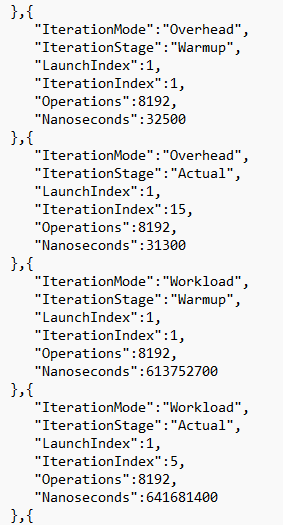
\includegraphics[width=0.3\textwidth]{../img/BenchmarkDotNET-modes.png}
    \caption{Struktura výsledků měření frameworku BenchmarkDotNET}
\end{figure}

BenchmarkDotNet je možné nakonfigurovat tak, aby se v~souboru s~výsledky nacházely podrobnosti o~prostředí, jako je operační systém,
verze platformy .NET, jméno, typ a~parametry procesoru. Dále aby se v~souboru s~výsledky nacházely
výsledky jednotlivých provedených měření. Výsledek měření u~sebe má informaci o~jméně
testovací metody, zpracované statistické údaje a~naměřené hodnoty z~různých módů a~iterací měření.
Konkrétní příklad toho, jak vypadají módy a~iterace měření se nachází na obrázku 2.1.
Názvy módů a~iterací mají intuitivní názvy, takže je z~nich poznat, kdy se ještě probíhá
překlad, a~kdy už se měří plně přeložený kód.

\subsection{Výstup měření JMH}

JMH je framework pro měření výkonu, který umožňuje pomocí anotací definovat výkonnostní testy
pro programy v~jazyce Java. Z~průzkumu \cite[]{unitTestingPerformanceSurvey} vyplývá, že se jedná o~nejpoužívanější framework
pro měření výkonu pro projekty vyvíjené v jazyce Java.

JMH obdobně jako BenchmarkDotNet poskytuje výsledek měření jako tabulku na standardní výstup.
Dále poskytuje výstup v~podobě strojově zpracovatelných formátů, jako jsou například XML
nebo JSON. O~výstup v~této podobě je nutné zažádat pomocí argumentů na~příkazové řádce při
spouštění měření. Další podrobnosti o~frameworku JMH je možné nalézt v~dokumentaci \cite[]{jmh}.

\begin{figure}[!ht]
    \centering
    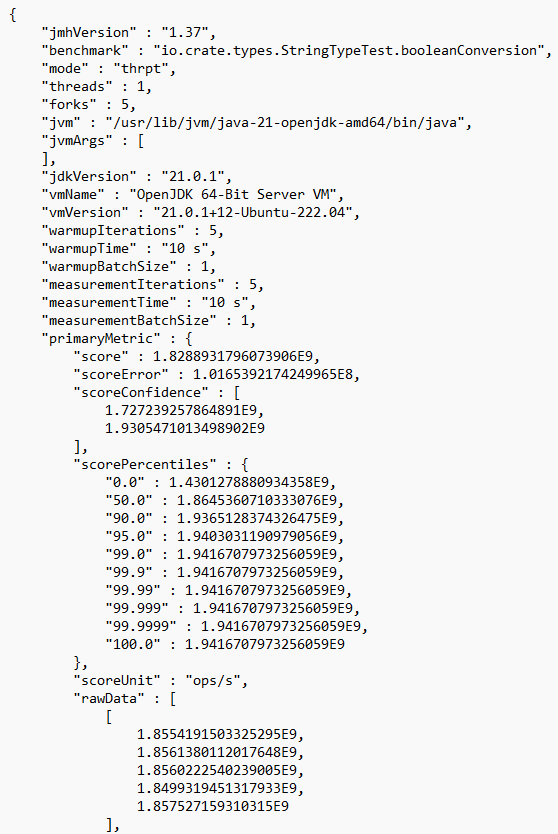
\includegraphics[width=0.6\textwidth]{../img/JMH-example.png}
    \caption{Struktura výsledků měření frameworku JMH}
\end{figure}

Ve výstupním souboru měření pomocí JMH lze nalézt informace o~stroji na~kterém probíhalo měření.
Jedná se především o~název stroje a~verzi operačního systému. Dále zde lze nalézt verzi Javy,
ve~které probíhalo měření. V~souboru je možné vidět také ostatní parametry měření, jako je
zahřívací doba a~počet zahřívacích iterací. Zahřívací iterace jsou zde uvedeny, protože Java
je stejně jako C\# jazyk kompilovaný metodou JIT. Je tedy nutné výstupní data vhodně filtrovat.

Jednotlivé naměřené hodnoty jsou ve výstupním souboru dostupné i~ve~výchozím nastavení JMH.
Naměřené hodnoty nejsou bezrozměrná čísla, ale jsou doplněny i~o~fyzikální jednotku,
kterou naměřená hodnota reprezentuje. Pro~každý běh (fork), přičemž běhů může být v~jednom
spuštění JMH více, se~objeví jedna sada měřených hodnot u~položky \lstinline|rawData|.

\section{Použití statistických metod pro analýzu dat}

Pro vyhodnocování výkonu je využito metod testování hypotéz. Ve statistickém testování
hypotéz se snažíme zamítnout nulovou hypotézu. V~případě zamítnutí nulové hypotézy
se předpokládá, že platí alternativní hypotéza. Popis testování hypotéz v této kapitole
se řídí skripty Pravděpodobnost a~statistika~1 \cite[]{samal_nmai059_nodate}.

Při testování hypotéz rozeznáváme
chyby I. a~II. druhu. Chyba I. druhu znamená, že jsme nulovou hypotézu zamítli,
i~když platí. Chyba II. druhu znamená, že jsme ji nezamítli, ale ona neplatí.

V našem případě porovnávání výkonu bude nulová hypotéza tvrzení, že výkon dvou verzí softwaru je stejný.
Jako alternativní hypotézu budeme uvažovat, že výkony dvou verzí softwaru jsou různé.
Pomocí metody testování hypotéz bude zjišťováno jestli mají dvě spojité náhodné veličiny stejnou střední hodnotu.
Hodnoty spojité náhodné veličiny jsou vždy hodnoty výkonu jedné testované metody programu jedné z verzí.
Pro každou z verzí je tedy uvažovaná jedna náhodná veličina.
Pokud hodnoty těchto veličin mají stejnou střední hodnotu, tak budeme tvrdit, že i výkon obou porovnávaných
verzí je stejný.

Chyba I. druhu tedy v našem případě znamená, že jsme prohlásili, že výkony dvou verzí jsou různé,
ačkoli jsou stejné. Pravděpodobnost chyby I. druhu je obvyklý parametr statistického testu.
Pravděpodobnost chyby I. druhu bude dále značen jako parametr $\alpha$. Parametr $\alpha$
je součástí konfigurace systému PerfEval.

\subsection{Welchův dvouvýběrový t-test}

Welchův dvouvýběrový t-test se používá jako statistika při testování hypotéz.
Tato statistika předpokládá, že náhodné veličiny jsou nezávislé a jejich rozdělení
se blíží normálnímu rozdělení. Nezávislost náhodných veličin je dána vlastnostmi
experimentu \cite[]{twosampletests} a její zajištění je mimo doménu řešeného problému. PerfEval
tedy v~případě použití možnosti t-test možnou závislost zanedbává.

Normalitě náhodných veličin je možné se přiblížit díky centrální limitní větě (CLV).
Se zajištěním normality nám pomůže samotná struktura naměřených výsledků. Výsledky měření
obsahují běhy. Běhy obsahují jednotlivé naměřené hodnoty. Naměřené hodnoty představují
vzorky náhodné veličiny. Pokud se budou v~rámci t-testu namísto naměřených hodnot uvažovat
průměry jednotlivých běhů, tak se podle CLV bude rozdělení těchto průměrů blížit normálnímu rozdělení.


Interval spolehlivosti pro Welchův t-test se spočítá podle následujícího algoritmu. V~algoritmu jsou
použité funkce, které odkazují na skutečně použité knihovní funkce. Funkce mean počítá střední hodnotu
sady hodnot. Funkce var počítá rozptyl sady hodnot. TDistribution je třída, která reprezentuje T-rozdělení
pro statistický test a~parametr konstruktoru je počet stupňů volnosti. Vzorec pro stupně volnosti je dostupný na~Wikipedii
Welchova t-testu \cite[]{enwiki:1184251732}. Vstupními parametry jsou vzorky náhodných veličin a parametr $\alpha$ (critValue.)

\begin{algorithm}[!ht]
    \caption{WelchCI}
    \KwIn{samples1, samples2, critValue}
    \KwOut{lowerBound, upperBound}

    n1 = length(samples1)\;
    n2 = length(samples2)\;

    mean1 = mean(samples1)\;
    mean2 = mean(samples2)\;

    var1 = var(samples1)\;
    var2 = var(samples2)\;

    varOverN1 = var1 / n1\;
    varOverN2 = var2 / n2\;

    degreesOfFreedom = Math.Pow(varOverN1 + varOverN2, 2) / (varOverN1 * varOverN1 / (N1-1) + varOverN2 * varOverN2 / (N2-2))\;

    tDist = new TDistribution(degreesOfFreedom)\;
    tCrit = tDist.inverseCumulativeProbability(critValue / 2)\;
    marginOfError = tCrit * Math.Sqrt(varOverN1 + varOverN2)\;

    lowerBound = mean1 - mean2 - marginOfError\;
    upperBound = mean1 - mean2 + marginOfError\;

\end{algorithm}

Nakonec se již jen zkoumá, zdali tento interval obsahuje nulu.
Pokud interval nulu neobsahuje, pak lze s~pravděpodobností $1-\alpha$ správně tvrdit, že
nulová hypotéza neplatí.

\subsection{Percentilový hierarchický bootstrap}

%% - https://www.youtube.com/watch?v=Xz0x-8-cgaQ

Bootstrap je statistická metoda využívající tzv. resamplování.
Stejně jako u~dvouvýběrového t-testu se předpokládá nezávislost náhodných veličin.
Podmínka nezávislosti bude zanedbána, protože ji není možné zaručit.
Bootstrap se jako metoda používá v~případě, kdy o~náhodných veličinách není možné
určit téměř žádné silné předpoklady. Díky této vlastnosti je bootstrap pro testování
hypotéz o~výkonu verzí softwaru použit.

\begin{algorithm}[!ht]
    \caption{Bootstrap1D}
    \KwIn{measurements, iterationCount}
    \KwOut{bootstrappedSamples}
    
    n = length(measurements)\;
    samples = []\;

    \For{i = 0; i < iterationCount; i += 1}{
        sum = 0\;
        \For{j = 0; j < n; j = j + 1}{
            index = random() mod n\;
            sum += measurements[index]\;
        }
        samples.add(sum/n)\;
    }
    
    \Return{samples}\;
\end{algorithm}

\begin{algorithm}[!ht]
    \caption{Bootstrap2D}
    \KwIn{runs1, runs2, iterationCount}
    \KwOut{bootstrappedSamples}
    
    n = length(runs1)\;
    m = length(runs2)\;
    samples = []\;
    
    \For{i = 0; i < iterationCount; i += 1}{
        samples1 = []\;
        \For{j = 0; j < n; j += 1}{
            index = random() mod n\;
            samples1.add(Bootstrap1D(runs1[index], 1))\;
            }
        samples2 = []\;
        \For{k = 0; k < m; k += 1}{
            index = random() mod m\;
            samples2.add(Bootstrap1D(runs2[index], 1))\;
        }
        diff = mean(samples1)-mean(samples2)\;
        samples.add(diff)\;
    }
    
    \Return{samples}\;
\end{algorithm}

Podle percentilového bootstrapu se interval spolehlivosti nalezne tak, že se hranice intervalu stanoví jako $\frac{\alpha}{2}$-tý
a~$\frac{1-\alpha}{2}$-tý percentil z~resamplovaného souboru. Tyto dvě hodnoty budou představovat hranice intervalu.

Zkoumanou náhodnou veličinou je rozdíl dvou náhodných veličin. Tyto dvě náhodné veličiny jsou dány měřením
výkonnosti dvou verzí softwaru. Nulová hypotéza, která je vyvracena, tvrdí, že obě veličiny mají stejnou střední hodnotu.
Pokud tedy interval spolehlivosti neobsahuje nulu, tak můžeme nulovou hypotézu vyvrátit, protože s~pravděpodobností
$1-\alpha$ o ní test správně prohlásil, že neplatí.

Naměřené vzorky však nejsou prostý statistický soubor. Jedná se o~hierarchický soubor dat.
Každé jedno měření se skládá z~jednoho, nebo více běhů. Každý běh se skládá z~jednoho, nebo více naměřených údajů.
Vytváření bootstrapového statistického souboru tedy vypadá trochu odlišně.

Bootstrap2D ukazuje, jak vypadá výběr nového statistického souboru. Vyberou
se náhodné běhy z~jednotlivých výsledků měření. Z těchto běhů se získá 1D bootstrap.
Novým prvkem vytvářeného statistického souboru se stane rozdíl těchto bootstrapů.

\subsection{Co dělat v případě nevyvrácení hypotézy?}

V~případě nevyvrácení nulové hypotézy nám statistické testy nedávají žádnou informaci.
Nicméně je stále nutné se rozhodnout, zdali nulová hypotéza platí. Je nutné se ale stále
vyvarovat chyby II. druhu. Proto v tomto případě budeme považovat nulovou hypotézu za platnou,
pokud bude interval spolehlivosti dostatečně úzký. Pokud má tedy interval spolehlivosti
dolní mez $D_{LOW}$ a horní mez $D_{HIGH}$, pak je jeho šířka $D_{HIGH}-D_{LOW}$. Odhadovaný průměr by byl $\frac{D_{HIGH}+D_{LOW}}{2}$.
Relativní šířka intervalu je tedy poměr šířky a průměru, tedy $\frac{2\cdot(D_{HIGH}-D_{LOW})}{D_{HIGH}+D_{LOW}}$.

V případě většího množství vzorků je možné zužovat interval spolehlivosti. Vztah mezi
šířkou a~počtem vzorků odpovídá $O(\frac{1}{\sqrt{n}})$, kde $n$ je počet vzorků. Z~daného
množství vzorků je tedy možné odhadnout, kolik vzorků je ještě zapotřebí změřit.

V případě, že je interval dostatečně úzký, prohlásíme, že nulová hypotéza platí.
V případě, že interval není dostatečně úzký, prohlásíme, že vzorků není dost.

PerfEval tedy v~konečném důsledku rozlišuje tři základní výsledky porovnání výkonu verzí.
Test končí s~kladným výsledkem, pokud platí nulová hypotéze dle kritérií výše. Test
končí s~kladným výsledkem také když je nulová hypotéza vyvrácena, ale výkon novější verze je lepší.
V~ostatních případech test neprojde. Další dva možné výsledky testu tedy budou značit selhání.
Druhý výsledek testu značí, že~nulová hypotéza neplatí, a~zároveň, že~došlo ke~zhoršení výkonu.
Třetí výsledek značí, že~se~nulovou hypotézu nepodařilo vyvrátit, ale~počet naměřených výsledků
je~příliš malý.

\chapter{Systém PerfEval}

Když už jsou známy požadavky na aplikaci, tak je možné začít ji navrhovat.
V~této kapitole jsou podrobně popsány úvahy a~rozhodnutí, které byly v~průběhu vývoje
provedeny. Jednotlivá rozhodnutí byla následně promítnuta do~architektury a~chování aplikace.

%\section{???}
%Výsledky testování výkonu se tedy musejí vyhodnocovat tak, že se podrobně prozkoumá výsledná sada čísel.
%Oproti testování korektnosti, kdy test projde nebo neprojde, je testování výkonu výrazně složitější.
%Pohledem na samostatnou sadu dat se nedá určit, zdali je software dostatečně rychlý. Aby bylo možné
%ze~sady určit něco vypovídajícího, bylo by možné stanovit pevný limit výkonnosti.
%Tento přístup nemusí být vypovídající při dlouhodobém vývoji
%a~při hodnotách hluboko pod limitem. Proto je vhodné, aby se datové sady, které testovací framework produkuje,
%porovnávaly mezi sebou. Porovnáním sad je totiž možné zjistit, jestli nedošlo k~významným změnám výkonu
%při~vývoji od~předchozí verze. Frameworky samotné však tuto možnost obvykle nemají.

\section{Analýza řešení}

\subsection{Měření výkonu}

Před začátkem vývoje PerfEvalu bylo nutné zamyslet nad tím, jak můžou výsledky měření výkonu softwaru vypadat.
V následujících odstavcích budou zmiňovány jednotlivé poznatky o~výsledcích měření výkonu.
Tyto poznatky vedly k~tomu, jak se PerfEval chová a~jakou má architekturu.

\medskip

\noindent\textbf{Měřené veličiny.} Jak jsme v první kapitole viděli, tak měřící
frameworky umožňují měřit mnoho různých fyzikálních veličin. Patří mezi ně například
doba vykonávání metody, frekvence počtu operací za jednotku času a spotřeba paměti.
Předpokládat se tedy dá jen to, že pokud vezmu dva výsledky měření výkonu ze~dvou různých
verzí, tak budou reprezentovány stejnou fyzikální veličinou a~v~lepším případě budou mít
i~stejnou fyzikální jednotku. Je tedy vhodné, aby výsledný systém byl schopen přijmout
jakoukoli veličinu bez ohledu na jednotku.

\medskip

\noindent\textbf{Identifikátory testů.} Protože testovací frameworky nepoužívají žádné identifikátory testů, tak je nejpřímější
řešení k~jejich rozpoznávání používat jména testovacích metod jako identifikátor. Tato jména poskytují ve~výsledcích
měření jak framework BenchmarkDotNet, tak framework JMH. Z~dokumentace frameworku Criterion \cite[]{criterion}
pro měření výkonu v~jazyce~Rust se název metody ve~výsledcích nachází také. Z~toho lze
usoudit, že použití jména metody jako identifikátoru může být dostatečně obecné.

\medskip

\noindent\textbf{Kompilace just-in-time.} V~případě měření výkonu u~jazyků, které jsou kompilované metodu JIT, je nutné být obezřetný. Je nutné
všímat si, jaká data byla naměřena. Jazyky kompilované metodou JIT mohou při měření podléhat tzv. zahřívací
fázi. Jedná se o~fázi, kdy kód ještě není plně optimalizovaný, ale již se provádí a~může být měřen.
V~závislosti na použitém měřícím frameworku je pak nutné naměřená data vhodně filtrovat. V~případě, že
by se data před a~po~optimalizaci nacházela v~jedné sadě dat, mohla by být zkreslená.

\subsection{Použití statistických metod pro analýzu dat}

\noindent\textbf{Výsledek měření.} S~testováním výkonu je problém. Když se spustí měření výkonu, tak výsledkem je pouhá
datová sada. Tato datová sada nevypovídá nic o~změně průběžného výkonu, která
je zajímavá. Právě podle změny ve~výkonu softwaru je možné zjistit, jestli je nutné
kód optimalizovat, protože dochází k~významným zhoršením.

\medskip

\noindent\textbf{Šum.} Při měření výkonu dochází jako při jakémkoli jiném měření k šumu. Tento šum se projevuje
tak, že pokud se měření opakuje při~stejných podmínkách, tak se naměřené hodnoty liší.
Tomuto šumu se nelze vyvarovat. Měření proto opakujeme a~naměřené hodnoty vyhodnocujeme
pomocí statistických metod, které si s~tímto šumem poradí.

\medskip

\noindent\textbf{Testování hypotéz.} Pro vyhodnocování výkonu je využito metod testování hypotéz. Ve statistickém testování
hypotéz se snažíme zamítnout nulovou hypotézu. V~případě zamítnutí nulové hypotézy
se předpokládá, že platí alternativní hypotéza. Popis testování hypotéz v této kapitole
se řídí skripty Pravděpodobnost a~statistika~1 \cite[]{samal_nmai059_nodate}.

Při testování hypotéz rozeznáváme
chyby I. a~II. druhu. Chyba I. druhu znamená, že jsme nulovou hypotézu zamítli,
i~když platí. Chyba II. druhu znamená, že jsme ji nezamítli, ale ona neplatí.

V našem případě porovnávání výkonu bude nulová hypotéza tvrzení, že výkon dvou verzí softwaru je stejný.
Jako alternativní hypotézu budeme uvažovat, že výkony dvou verzí softwaru jsou různé.
Pomocí metody testování hypotéz bude zjišťováno jestli mají dvě spojité náhodné veličiny stejnou střední hodnotu.
Hodnoty spojité náhodné veličiny jsou vždy hodnoty výkonu jedné testované metody programu jedné z verzí.
Pro každou z verzí je tedy uvažovaná jedna náhodná veličina.
Pokud hodnoty těchto veličin mají stejnou střední hodnotu, tak budeme tvrdit, že i výkon obou porovnávaných
verzí je stejný.

Chyba I. druhu tedy v našem případě znamená, že jsme prohlásili, že výkony dvou verzí jsou různé,
ačkoli jsou stejné. Pravděpodobnost chyby I. druhu je obvyklý parametr statistického testu.
Pravděpodobnost chyby I. druhu bude dále značen jako parametr $\alpha$. Parametr $\alpha$
je součástí konfigurace systému PerfEval.

Následující dvě podkapitoly popisují vybrané statistické testy, které jsou využity v~systému PerfEval.
Dvouvýběrový Welchův t-test byl vybrán, protože t-test se podle \cite[]{samal_nmai059_nodate} používá pro porovnání
středních hodnot dvou náhodných veličin. Welchův t-test byl vybrán, protože oproti Studentovu t-testu nevyžaduje
stejné rozptyly porovnávaných náhodných veličin. Percentilový hierarchický bootstrap byl vybrán, protože
je vhodný v~situaci, kdy není možné předpokládat normální rozdělení dat.
Poslední podkapitola popisuje jakým způsobem se řeší nevyvrácení nulové hypotézy.

\subsubsection{Welchův dvouvýběrový t-test}

Welchův dvouvýběrový t-test se používá jako testová statistika při testování hypotéz.
Tato statistika předpokládá, že náhodné veličiny jsou nezávislé a jejich rozdělení
se blíží normálnímu rozdělení. Nezávislost náhodných veličin je dána vlastnostmi
experimentu \cite[]{twosampletests} a její zajištění je mimo doménu řešeného problému. PerfEval
tedy v~případě použití možnosti t-test možnou závislost zanedbává.

Normalitě náhodných veličin je možné se přiblížit díky centrální limitní větě (CLV).
Se zajištěním normality nám pomůže samotná struktura naměřených výsledků. Výsledky měření
obsahují běhy. Běhy obsahují jednotlivé naměřené hodnoty. Naměřené hodnoty představují
vzorky náhodné veličiny. Pokud se budou v~rámci t-testu namísto naměřených hodnot uvažovat
průměry jednotlivých běhů, tak se podle CLV bude rozdělení těchto průměrů blížit normálnímu rozdělení.

Interval spolehlivosti pro Welchův t-test se spočítá podle dále uvedených vzorců.
Postupně se počítají stupně volnosti, kritická hodnota t-rozdělení, chybovost, dolní a~horní mez intervalu.
Vzorec pro výpočet stupňů volnosti je převzatý z~Wikipedie Welchova t-testu \cite[]{enwiki:1184251732}.
Ostatní vzorce jsou převzaty ze skript \cite[]{samal_nmai059_nodate}.

\begin{equation*}
    \bar{X_i} = \frac{1}{n_i} \sum_{j=1}^{n_i} X_{ij}
\end{equation*}

\begin{equation*}
    s_i^2 = \frac{1}{n_i-1} \sum_{j=1}^{n_i} (X_{ij} - \bar{X_i})^2
\end{equation*}

\begin{equation*} \label{eq:welch_df}
    df = \frac{(\frac{s_1^2}{n_1} + \frac{s_2^2}{n_2})^2}{\frac{s_1^4}{n_1^2(n_1-1)} + \frac{s_2^4}{n_2^2(n_2-1)}}
\end{equation*}

\begin{equation*}
    t = \psi_{df}^{-1}(1-\frac{\alpha}{2})
\end{equation*}

\begin{equation*}
    marginOfError = t \cdot \sqrt{\frac{s_1^2}{n_1} + \frac{s_2^2}{n_2}}
\end{equation*}

\begin{equation*}
    lowerBound = \bar{X_1} - \bar{X_2} - marginOfError
\end{equation*}

\begin{equation*}
    upperBound = \bar{X_1} - \bar{X_2} + marginOfError
\end{equation*}

Použité značení:
\begin{itemize}
    \item $df$ - stupně volnosti
    \item $s_1^2$ - výběrový rozptyl první sady vzorků
    \item $s_2^2$ - výběrový rozptyl druhé sady vzorků
    \item $n_1$ - počet prvků první sady vzorků
    \item $n_2$ - počet prvků druhé sady vzorků
    \item $t$ - kritická hodnota t-rozdělení
    \item $\psi_{df}^{-1}$ - inverzní distribuční funkce t-rozdělení
    \item $\bar{X}_1$ - výběrový průměr první sady vzorků
    \item $\bar{X}_2$ - výběrový průměr druhé sady vzorku
\end{itemize}


%\begin{algorithm}[!ht]
%    \caption{WelchCI}
%    \KwIn{samples1, samples2, critValue}
%    \KwOut{lowerBound, upperBound}
%
%    n1 = length(samples1)\;
%    n2 = length(samples2)\;
%
%    mean1 = mean(samples1)\;
%    mean2 = mean(samples2)\;
%
%    var1 = var(samples1)\;
%    var2 = var(samples2)\;
%
%    varOverN1 = var1 / n1\;
%    varOverN2 = var2 / n2\;
%
%    degreesOfFreedom = Math.Pow(varOverN1 + varOverN2, 2) / (varOverN1 * varOverN1 / (N1-1) + varOverN2 * varOverN2 / (N2-2))\;
%
%    tDist = new TDistribution(degreesOfFreedom)\;
%    tCrit = tDist.inverseCumulativeProbability(critValue / 2)\;
%    marginOfError = tCrit * Math.Sqrt(varOverN1 + varOverN2)\;
%
%    lowerBound = mean1 - mean2 - marginOfError\;
%    upperBound = mean1 - mean2 + marginOfError\;
%
%\end{algorithm}

Nakonec se již jen zkoumá, zdali tento interval obsahuje nulu.
Pokud interval nulu neobsahuje, pak lze s~pravděpodobností $1-\alpha$ správně tvrdit, že
nulová hypotéza neplatí.

\subsubsection{Percentilový hierarchický bootstrap}

%% - https://www.youtube.com/watch?v=Xz0x-8-cgaQ

Bootstrap je statistická metoda využívající tzv. resamplování.
Stejně jako u~dvouvýběrového t-testu se předpokládá nezávislost náhodných veličin.
Podmínka nezávislosti bude zanedbána, protože ji není možné zaručit.
Bootstrap se jako metoda používá v~případě, kdy o~náhodných veličinách není možné
určit téměř žádné silné předpoklady. Díky této vlastnosti je bootstrap pro testování
hypotéz o~výkonu verzí softwaru použit.

\begin{algorithm}[!ht]
    \caption{MeanBootstrap1D}
    \KwIn{measurements, replicationCount}
    \KwOut{bootstrappedSamples}
    
    n = length(measurements)\;
    samples = []\;

    \For{i = 0; i < replicationCount; i += 1}{
        resampledSamples = []\;
        \For{j = 0; j < n; j = j + 1}{
            index = random() mod n\;
            resampledSamples.add(measurements[index])\;
        }
        samples.add(mean(resampledSamples))\;
    }
    
    \Return{samples}\;
\end{algorithm}

\begin{algorithm}[!ht]
    \caption{MeanBootstrap2D}
    \KwIn{runs1, runs2, replicationCount}
    \KwOut{bootstrappedSamples}
    
    n = length(runs1)\;
    m = length(runs2)\;
    samples = []\;
    
    \For{i = 0; i < replicationCount; i += 1}{
        samples1 = []\;
        \For{j = 0; j < n; j += 1}{
            index = random() mod n\;
            samples1.add(MeanBootstrap1D(runs1[index], 1))[0]\;
            }
        samples2 = []\;
        \For{k = 0; k < m; k += 1}{
            index = random() mod m\;
            samples2.add(MeanBootstrap1D(runs2[index], 1))[0]\;
        }
        diff = mean(samples1)-mean(samples2)\;
        samples.add(diff)\;
    }
    
    \Return{samples}\;
\end{algorithm}

Podle percentilového bootstrapu se interval spolehlivosti nalezne tak, že se hranice intervalu stanoví jako $\frac{\alpha}{2}$-tý
a~$\frac{1-\alpha}{2}$-tý percentil z~resamplovaného souboru. Tyto dvě hodnoty budou představovat hranice intervalu.

Zkoumanou náhodnou veličinou je rozdíl dvou náhodných veličin. Tyto dvě náhodné veličiny jsou dány měřením
výkonnosti dvou verzí softwaru. Nulová hypotéza, která je vyvracena, tvrdí, že obě veličiny mají stejnou střední hodnotu.
Pokud tedy interval spolehlivosti neobsahuje nulu, tak můžeme nulovou hypotézu vyvrátit, protože s~pravděpodobností
$1-\alpha$ o ní test správně prohlásil, že neplatí.

Naměřené vzorky však nejsou prostý statistický soubor. Jedná se o~hierarchický soubor dat.
Každé jedno měření se skládá z~jednoho, nebo více běhů. Každý běh se skládá z~jednoho, nebo více naměřených údajů.
Vytváření bootstrapového statistického souboru tedy vypadá trochu odlišně.

MeanBootstrap2D ukazuje, jak vypadá výběr nového statistického souboru. Vyberou
se náhodné běhy z~jednotlivých výsledků měření. Z~těchto běhů se získá 1D bootstrap.
Novým prvkem vytvářeného statistického souboru se stane rozdíl těchto bootstrapů.

\subsubsection{Co dělat v případě nevyvrácení hypotézy?}

V~případě nevyvrácení nulové hypotézy nám statistické testy nedávají žádnou informaci.
I~přes tuto vlastnost statistických testů, je pro praktické užití nutné se rozhodnout, zdali
změnu výkonu hlásit. Stále je nutné se vyvarovat chyby II. druhu. Proto v~tomto případě nebudeme hlásit zhoršení výkonu,
pokud bude získaný interval spolehlivosti dostatečně úzký. Pokud má tedy interval spolehlivosti
dolní mez $D_{LOW}$ a horní mez $D_{HIGH}$, pak je jeho šířka $D_{HIGH}-D_{LOW}$. Odhadovaný průměr by byl $\frac{D_{HIGH}+D_{LOW}}{2}$.
Relativní šířka intervalu je tedy poměr šířky a průměru, tedy $\frac{2\cdot(D_{HIGH}-D_{LOW})}{D_{HIGH}+D_{LOW}}$.

V případě většího množství vzorků je možné zužovat interval spolehlivosti. Vztah mezi
šířkou a~počtem vzorků odpovídá $O(\frac{1}{\sqrt{n}})$, kde $n$ je počet vzorků. Z~daného
množství vzorků je tedy možné odhadnout, kolik vzorků je ještě zapotřebí změřit.

V~případě, že je interval dostatečně úzký, nebudeme zhoršení výkonu hlásit a~řekneme, že výkon obou verzí je stejný.
V~případě, že interval není dostatečně úzký, prohlásíme, že vzorků není dost.

PerfEval tedy v~konečném důsledku rozlišuje tři základní výsledky porovnání výkonu verzí.
Test nahlásí zhoršení výkonu právě tehdy, když bude nulová hypotéza vyvrácena a~zároveň
bude průměrný výkon novější verze horší než průměrný výkon starší verze.
Test nenahlásí žádnou změnu výkonu, pokud nulová hypotéza nebyla vyvrácena a~interval spolehlivosti
bude dostatečně úzký. V~případě, že nulová hypotéza nebyla vyvrácena a~interval spolehlivosti
je příliš široký, test nahlásí, že vzorků není dostatečné množství.

\subsection{Použité statistické metody}
Pro porovnání dvou výsledků měření se používají statistické metody. Statistické metody se používají k~zjištění,
jestli výsledky měření považované za~náhodné veličiny mají stejnou střední hodnotu a~jestli je vzorků dostatečné množství.
V~předchozí kapitole byly popsány dvě statistické metody, které jsou v~systému PerfEval implementovány.
Jedná se o~metody \textbf{bootstrap} a~\textbf{t-test}.

\medskip

\noindent\textbf{Bootstrap.} Výhodou bootstrapu je, že není vyžadovaný předpoklad normálního rozdělení dat.
Bootstrap je implementován pomocí algoritmů z~předchozí podkapitoly. Je tedy patrné, že výpočet je pomalý,
protože dochází k~velkému množství náhodných výběrů z~dvoudimenzionální sady dat. Pokud má uživatel
dostatečné množství času měl by této metodě dát přednost právě kvůli tomu, že není vyžadován předpoklad normálního rozdělení dat.
Jak již bylo řečeno, tak zajištění normality dat je totiž mimo doménu řešeného problému.

\medskip

\noindent\textbf{T-test.} T-test je použitý ve variantě Welchova t-testu. Tento test je výhodný tím, že je rychlejší než bootstrap.
Rychlejší je proto, že se jedná o pouhé dosazení hodnot do vzorců. Nevýhodou je, že je vyžadován předpoklad normálního rozdělení dat.
Tento předpoklad však není zaručen, a tudíž může dojít k~zkreslení výsledků. T-test je tedy vhodný pro případy, kdy je množství naměřených
vzorků velké a~uživatel má málo času na~vyhodnocení výsledků.

\subsection{Spouštění testů systémem PerfEval}
V~počátku vývoje bylo nutné se~rozhodnout, jakým způsobem bude systém přijímat a~zpracovávat výsledky testů.
V~úvahu přicházela varianta \textbf{Měření výkonu uživatelem}, že~uživatel provede měření výkonu sám. Druhá varianta byla \textbf{Měření výkonu PerfEvalem} tak,
že~uživatel systému vysvětlí, jakým způsobem se~testování výkonu spouští. Pokud by byla zvolena tato varianta,
tak by bylo nutné nalézt dostatečně univerzální způsob spouštění testů.

\medskip

\noindent\textbf{Měření výkonu PerfEvalem.} Aplikace a~benchmarky pro měření výkonu mohou být jak konzolové, tak grafické aplikace. Pokud by PerfEval měl
měření provádět sám, tak by téměř určitě nebyl schopen pracovat s~grafickými aplikacemi, ale byl by schopen
spouštět programy s~parametry na~příkazové řádce.

Dále by bylo nutné vysvětlit, jak vypadá výstup spouštěných testů. Když pomineme formát, tak je nutné zjistit,
kam program, který provádí měření, výsledky ukládá. Benchmarkovací systém BenchmarkDotNet například vypisuje
výsledky měření v podobě tabulky na standardní výstup a~zároveň ukládá strojově čitelné výsledky do~speciálního
k~tomu určeného adresáře.

Pokud by PerfEval využíval této varianty, tak by uživatel při inicializaci systému musel zadat, jak spustit testy
a~kam se uloží výsledek. Tímto způsobem by došlo k~tomu, že PerfEval by začal určovat, jak mají vypadat programy,
jejichž výstupy přijímá.
\medskip
\noindent\textbf{Měření výkonu uživatelem.} V této variantě tedy uživatel spouští testy sám a~PerfEval pouze porovnává výsledky.
Při inicializaci uživatel oproti předchozí variantě pouze vybere vhodný parser. Zvolený parser umí zpracovat příslušný formát dat z~benchmarkovacího frameworku,
který uživatel používá. Toto řešení bylo vybráno a~implementováno v~systému PerfEval.

Vybrané řešení tedy od uživatele požaduje krok navíc. Nicméně dává uživateli mnohem větší prostor pro to, jak
spouští testy a~kam ukládá výsledky. O~tom, že existují výsledky měření dané verze, a kde se nachází, uživatel
pouze informuje PerfEval. Systém tak ani do budoucna neklade žádné nároky na to, jak má uživatel testy spouštět,
ani kde se mají výsledky ukládat.

\subsection{Rozpoznání formátu výsledků měření}

Systém, který porovnává výsledky měření výkonu, by měl mít informace o~tom v~jakém formátu jsou data uložena
a~který benchmarkovací framework je vytvořil. Podle použitého frameworku a~formátu je totiž možné výsledky
měření zpracovat pomocí programu a~transformovat data o~měření tak, aby jim systém rozuměl.
Problém je tedy v tom, jak se systém dozví o~tomto formátu a~o~použitém frameworku.

Nejpříjemnější řešení pro uživatele by bylo, že by systém sám přišel na to, který framework a~formát je použitý.
Uživatel by totiž nemusel vědět pomocí jakého frameworku a~v~jakém formátu data ukládá. Pro systém by však mohl
být problém různé frameworky rozlišit.

Při rozlišování by se totiž musel podívat do~dat uložených v souboru
a~na~základě obsahu určit o~jaký formát a~framework se jedná. Správné určení frameworku a~formátu by bylo zásadní pro
správnou reprezentaci dat. Samotné rozlišování frameworků a~formátu by bylo obtížné, protože soubory s~výsledky
měření obsahují podobná data a~položky, ale hierarchie struktur ve~kterých jsou uloženy jsou různé.
Při následném rozlišování většího množství formátů a~frameworků by tedy systém automatického rozpoznávání
začal být příliš komplikovaný, aby si zachoval přesnost.

Docházelo by také k~dvojímu čtení souboru z~paměti. První čtení souboru by sloužilo k rozpoznání formátu,
aby systém zjistil, jak má data ze souboru zpracovávat. Při druhém čtení souboru by již transformoval data
tak, aby jim rozuměla vyhodnocovací část systému.

PerfEval tedy řeší tento problém tak, že uživatel při inicializaci zadá jméno jednoho z~dostupných parserů.
Předpokládá se tedy, že pokud uživatel používá výkonnostní testy, tak framework a~výstupní formát je shodný s~těmi které zvolený parser rozpoznává.
Pokud má PerfEval parser pro tento framework a~formát dat parser, pak je schopný vyhodnocovat výsledky měření.
V~opačném případě si tento parser může uživatel doimplementovat.

Tento přístup umožňuje snazší implementaci nových parserů. Není totiž nutné k těmto parserům implementovat
také sadu pravidel, kdy má být použitý. Uživatele tento přístup omezuje v tom, že musí znát framework a~formát
ve~kterém se výsledky měření nachází. Protože psaní výkonnostních testů není jednoduché, tak lze předpokládat,
že uživatel je dostatečně zkušený, aby tuto znalost měl.

\subsection{Kdy zpracovávat naměřená data?}

Systém musí v~některém bodě výpočtu zpracovat data z~měření. Existuje několik možností, kdy
je možné toto zpracování do formátu, kterému bude rozumět, udělat. Je možné buď zpracovat
data ihned po tom, co se systém dozví o~jejich existenci, nebo až těsně před vyhodnocováním.

Pokud by se data zpracovávala hned po tom, co se o nich systém dozví, tak to nutně neznamená,
že již má proběhnout vyhodnocování. Je tedy nutné zvolit nějaký formát do kterého zpracovaná data
uložit. Při vyhodnocení by se pak data z~tohoto formátu musela opět zpracovat. Tento způsob
zpracování dat by měl význam pouze v~případě, že by první předzpracování vedlo k~velkému
zrychlení druhého zpracování. Zároveň by toto řešení vedlo k~dvojímu ukládání dat, protože
by někde byl uložený původní výsledek měření v původním formátu, a~také soubor se~předzpracovanými
výsledky měření, který by obsahoval data se~stejným významem.

Výše zmíněné nevýhody vedly k tomu, že systém zpracovává data z~původního formátu těsně před
vyhodnocováním. Podle zvoleného parseru se tedy data naparsují těsně před vyhodnocením ze~souborů,
které vygeneroval přímo framework pro měření výkonu.

\subsection{Jak přistupovat k naměřeným datům?}

Systém, který porovnává výsledky měření, by měl mít nějaké informace o~tom, k~jaké verzi se měření vztahuje, nebo kde
se soubor s~výsledky nachází. Proto bylo při vývoji nutné se zamyslet nad tím, jakými způsoby lze tyto informace získat a~spravovat.
Systém PerfEval potřebuje o~výsledcích měření vědět, kde jsou uloženy a~ke~které verzi softwaru bylo měření provedeno.

\noindent\textbf{Složka s výsledky měření.} První zvažovaná varianta byla, že by existovala složka, do~které by uživatel vkládal výsledky měření. Tento adresář by byl určený
systémem PerfEval, nebo by byla zadaná cesta k~němu při inicializaci systému. Po~každém měření by tedy uživatel výsledek pouze
vložil do~správné složky a~o~nic víc by se nemusel starat.

Toto řešení má několik nevýhod. Omezuje uživatele v~tom, jak musí výsledky testů ukládat. Dále by se špatně určovalo,
ke~které verzi bylo měření provedeno, protože toto se ve~výsledcích měření běžnými frameworky neudává. Pravděpodobně by proto
vznikla hierarchie v tomto adresáři a~uživatel by například pomocí pojmenovávání složek určoval, ke~které verzi se měření vztahuje.

Celkově tedy tento způsob poskytuje jednoduché zjištění, kde se výsledek testu nachází. Je to pevně dané. Není ale možné jednoduše
zjistit verzi, protože je nutné projít adresářovou strukturu, což může být při velkém množství dat pomalé.

\medskip

\noindent\textbf{Cache a~složka s~výsledky měření.} Druhé uvažované řešení bylo vylepšení prvního řešení o~cache a sledování času modifikace adresářů.
Verze se totiž dobře určují při vkládání,
ale špatně dohledávají. Pravděpodobně by se používání některých verzí k~porovnání opakovalo častěji než u~jiných.
Zároveň pokud by nejnovější verze nebyla v cache, tak by se dohledávala postupným průchodem na základě nejmladšího data změny adresáře
v~adresáři s~výsledky měření. Cache by byla tvořena posledními několika desítkami naposledy použitých záznamů s~cestou k~výsledkům měření a~verzí.

Toto řešení má ale podobné nevýhody jako první. V~případě, že se verze porovnává poprvé, tak záznamy o~ní jistě nejsou v~cache
a~musí se prohledat adresářová struktura. Pokud je poslední úprava cache starší než nejnovější úprava nějakého podadresáře v~adresáři
s~výsledky měření, tak je nutné tuto část adresářové struktury projít. V~procházené části adresářové struktury je vždy nutné prozkoumat
zdali se jedná o~soubor verze, která je v cache, a~tak by se do ní měl přidat záznam o~tomto souboru. Popsaná práce s~cache měla
za~následek poslední uvažované řešení, kde již nezáleží na tom, kde jsou uložené výsledky měření. Jediné, co budeme předpokládat, je,
že uživatel soubory s~výsledky měření nepřesouvá.

\medskip

\noindent\textbf{Databáze s metadaty o~výsledcích měření.} Poslední uvažované řešení je strukturované ukládání metadat o~výsledcích měření. Využije se databáze o~jedné tabulce, kde
je uvedena cesta k~výsledku měření a~verze ke které byl výsledek změřen. Uživatel do~systému nahlásí, že má nový výsledek
měření, kde je uložen, a~k~jaké verzi softwaru je měření provedeno. Systém si tato data pouze poznamená do~databáze. Při
vyhodnocení pak pomocí databázových dotazů nalezen snadno všechny soubory s~výsledky měření k~potřebné verzi.

Toto řešení poskytuje jak rychlé vkládání nových výsledků, tak rychlé vyhledávání výsledků měření k~dané verzi.
Díky těmto vlastnostem bylo vybráno a~implementováno v~systému PerfEval.

\subsection{Formát výstupu}

Při volbě formátu v~jakém se budou výsledky výkonnostních testů prezentovat je nutné se zamyslet nad tím, kdo je bude číst a~zpracovávat.
Výsledky vyhodnocení bude zpracovávat zejména člověk a~průběžná integrace v~rámci verzovacího nástroje Git.

Pro člověka je čitelný formát zpracovaných dat tabulka s údaji o~tom, který test prošel a~který ne.
Jeden z~výstupních formátu systému PerfEval je takováto tabulka na příkazové řádce. Druhý formát s daty čitelnými pro člověka je
tabulka na HTML stránce, kterou PerfEval umí vygenerovat. Výstup v~HTML formátu je výhodný, protože je možné
soubor s~výsledky otevřít v~internetovém prohlížeči, který je dnes dostupný téměř na každém zařízení.

Strojem čitelný formát je XML soubor. XML má formát shodný s JUNIT XML formátem, který je běžně používaný v~průběžné integraci
při hlášení výsledků unit testů. Druhým zvoleným formátem je JSON, který je dnes běžně používaný pro serializaci dat v~různých
programovacích jazycích. Umožňuje tak snadnou integraci s dalšími programy.

\section{Architektura systému PerfEval}

Tato kapitola se věnuje popisu konkrétní architektury systému PerfEval.
Popisuje jakým způsobem jsou jednotlivé části systému navrženy a~jak spolu vzájemně interagují.

Samotné vyhodnocování jakožto porovnání dvou výsledků měření jedné sady testů výkonu je proces, který lze rozdělit do~několika kroků.
Zpracování dat uložených v souborech s výsledky měření až po vypsání výsledků vyhodnocení probíhá následujícím způsobem:

\begin{enumerate}
    \item Načtení a naparsování výsledků měření ze~souborů.
    \item Pomocí statistického testu porovnat dvě sady naměřených dat.
    \item Výsledek porovnání vypsat uživateli.
\end{enumerate}

\begin{figure}[!ht]
    \centering
    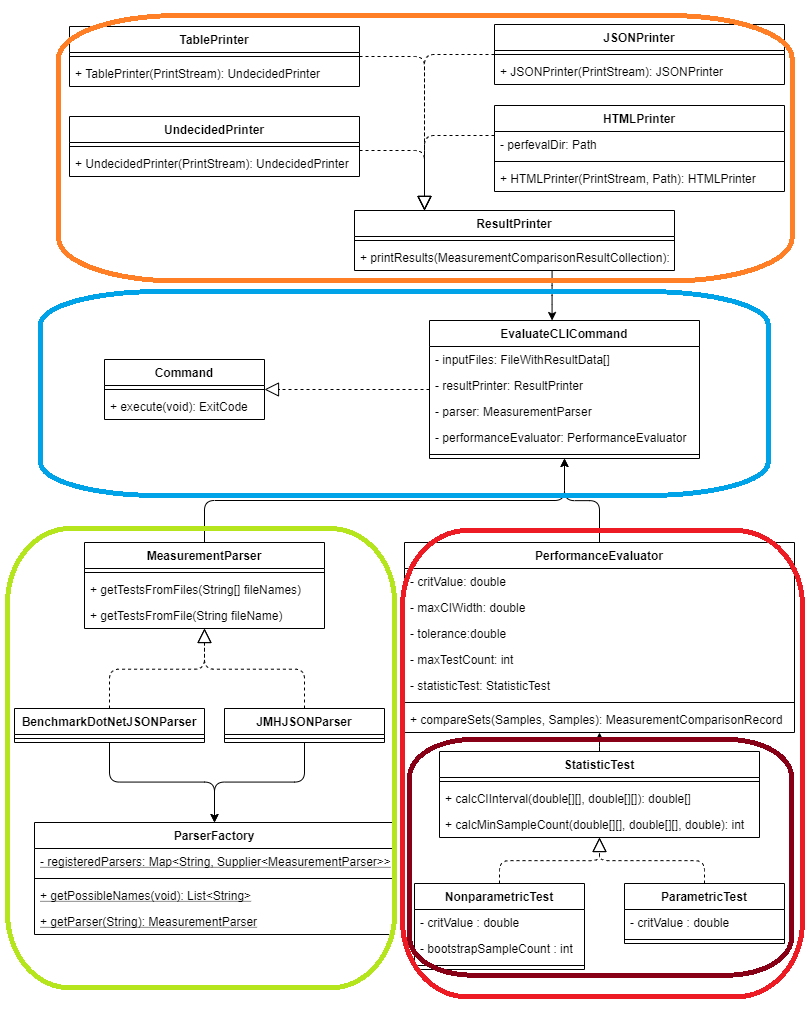
\includegraphics[width=0.92\textwidth]{../img/perfeval_evaluate_rect.png}
    \caption{Objektový návrh části PerfEvalu pro porovnávání výsledků měření}
\end{figure}

Obrázek 3.1 ukazuje rozdělení architektury vyhodnocovací části systému PerfEval do~čtyř logických celků.
Jedná se o logické celky, které se starají o~jednotlivé kroky vyhodnocování výsledků měření.

Na obrázku je vidět část systému kolem rozhraní \lstinline|MeasurementParser|, která se stará o~parsování výsledků měření.
Implementace tohoto rozhraní se stará o~načtení a~zpracování výsledků měření ze~vstupních souborů.
Produkují tak objekty, které reprezentují výsledky měření a~kterým rozumí zbytek systému.
Jednotlivé implementace tohoto rozhraní jsou závislé na~formátu výstupu frameworku, který byl použit pro měření výkonu.
Na základě konfigurace systému PerfEval vybere \lstinline|ParserFactory| správnou implementaci \lstinline|MeasurementParser|.

Obrázek dále znázorňuje třídu \lstinline|PerformanceEvaluator|, která se stará o~porovnání dvou instancí třídy \lstinline|Samples|.
Porovnání obstarává implementace rozhraní \lstinline|StatisticTest|. Volba implementace je dána parametry příkazové řádky.

Výsledky porovnání jsou následně vypsány uživateli pomocí implementace rozhraní \lstinline|ResultPrinter|.
Zvolená implementace tohoto rozhraní určuje formát výstupu, ve kterém jsou výsledky porovnání vypsány.
Volba implementace je dána parametry příkazové řádky.

Poslední částí, která je na obrázku 3.1 znázorněna, je hlavní třída celého vyhodnocování \lstinline|EvaluateCLICommand|.
Tato třída je implementací rozhraní \lstinline|Command|. Metoda \lstinline|execute| této třídy
provádí vyhodnocování podle popsaných kroků. Způsob provádění jednotlivých kroků je dané
dodanými implementacemi rozhraní \lstinline|MeasurementParser|, \lstinline|StatisticTest| a~\lstinline|ResultPrinter|.
Tyto implementace jsou předány při konstrukci třídy \lstinline|EvaluateCLICommand|.

Po vypsání výsledků porovnání se podle voleb z~konfiguračního souboru již jen nastaví exit kód programu a~ukončí se vyhodnocování.
Konfigurační soubor určuje jestli se mimo zhoršení výkonu hlásí také zlepšení výkonu a~nemožnost doměření dostatečného množství vzorků.

Samotná architektura systému je tedy postavena na rozhraních, které obklopují třídu \lstinline|EvaluateCLICommand|.
Pomocí nových implementací těchto rozhraní je možné systém rozšiřovat o~nové možnosti zpracování výsledků měření.
Architektura dále umožňuje snadné rozšíření o~nové formáty vstupu i~výstupu. Systém byl navržen tak, aby bylo
jednoduché změnit způsob provádění jednotlivých kroků vyhodnocování. Změna kroků samotných by vyžadovala
větší zásah do~architektury systému a~byla by složitá.



\chapter{Uživatelská dokumentace systému PerfEval}

\section{Instalace}

TODO: dodat, až se to bude vědět

\section{Dostupné příkazy}

Tato část práce se~zabývá jednotlivými příkazy systému PerfEval a jejich parametry.
V~jednotlivých podkapitolách je vysvětleno, k~čemu se daný příkaz používá. V~podkapitolách
se nachází také informace o~volitelných a~povinných parametrech jednotlivých příkazů.

\subsection{Příkaz init}

Příkaz init slouží k~inicializaci systému v~rámci aktuálního pracovního adresáře.
Systém PerfEval po~spuštění hledá v~pracovním adresáři složku s~názvem .performance. Pokud složka
není nalezena a~nebyl zadán příkaz init, končí s~chybou, že systém není inicializovaný.

\subsection*{Povinné argumenty:}
\begin{itemize}[label=\texttt{\textbf{\textendash}}]
    \item[\texttt{benchmark-parser}] Nastavení parseru, který se bude pro tento projekt používat.
        Jméno parseru je zadávané jako parametr tohoto příznaku.
        Parser se volí podle použitého testovacího frameworku a~výstupního formátu.
        Jedná se o~jediný parametr konfiguračního souboru, který lze zadat při inicializaci.
        Důvodem je, že je to jediný konfigurační parametr, jehož hodnotu není možné nastavit nějakým výchozím způsobem.
        Určuje totiž podobu a~formát vstupních dat, které PerfEval očekává.
\end{itemize}

\subsection*{Volitelné argumenty:}
\begin{itemize}[label=\texttt{\textbf{\textendash}}]
    \item[\texttt{force}] Příznak, který vynutí inicializaci i v případě, že je systém v adresáři již inicializovaný.
\end{itemize}

\subsection{Příkaz index-new-result}

Příkaz index-new-result slouží k~přidání výsledků měření výkonu do~databáze. Databáze
je pro~každý projekt zvlášť a~je tedy možné na~jednom zařízení systémem PerfEval spravovat více projektů.
Při přidávání informací o souboru s výsledky je nutné zadat cestu k tomuto souboru.
Verze, ke~které byly výsledky změřeny, může být zadaná také, nebo ji systém zkusí určit
podle git repozitáře.

\subsection*{Povinné argumenty:}
\begin{itemize}[label=\texttt{\textbf{\textendash}}]
    \item[\texttt{path}] Parametr tohoto příznaku udává cestu k~souboru s~výsledky měření.
\end{itemize}

\subsection*{Volitelné argumenty:}
\begin{itemize}[label=\texttt{\textbf{\textendash}}]
    \item[\texttt{version}] Parametr tohoto příznaku udává textovou reprezentaci verze SW, která se měřila.
    \item[\texttt{tag}] Parametr tohoto příznaku udává tag verze měření.
\end{itemize}

\subsection{Příkaz index-all-results}

Příkaz index-all-results slouží k~přidání více výsledků měření výkonu do~databáze.
Při přidávání informací o~souborech s~výsledky je nutné zadat cestu k~adresáři s~těmito výsledky.
Budou přidány všechny (i~zanořené) soubory v~tomto adresáři.
Verze, ke~které byly výsledky změřeny, může být zadaná také, nebo ji systém zkusí odhadnout
podle git repozitáře.

\subsection*{Povinné argumenty:}
\begin{itemize}[label=\texttt{\textbf{\textendash}}]
    \item[\texttt{path}] Parametr tohoto příznaku udává cestu k adresáři s výsledky měření.
\end{itemize}

\subsection*{Volitelné argumenty:}
\begin{itemize}[label=\texttt{\textbf{\textendash}}]
    \item[\texttt{version}] Parametr tohoto příznaku udává textovou reprezentaci verze SW, která se měřila.
    \item[\texttt{tag}] Parametr tohoto příznaku udává tag verze měření.
\end{itemize}

\subsection{Příkaz evaluate}

Příkaz evaluate porovnává dvě poslední zaznamenané verze, které byly změřeny.
Verze k~porovnání je možné specifikovat také manuálně pomocí příznaků. Výstupem
je tabulka nebo JSON s~výsledky porovnání. V~případě, že alespoň u~jednoho porovnání
došlo ke~zhoršení výkonu, bude selhání signalizováno exit kódem 1.

\subsection*{Volitelné argumenty:}
\begin{itemize}[label=\texttt{\textbf{\textendash}}]
    \item[\texttt{new-version}] Parametr udává textovou reprezentaci verze, která se má při porovnání považovat za~novější.
    \item[\texttt{new-tag}]     Pouze soubory s~tímto tagem budou použity k~porovnání jako novější.
    \item[\texttt{old-version}] Parametr udává textovou reprezentaci verze, která se má při porovnání považovat za~starší.
    \item[\texttt{old-tag}]     Pouze soubory s~tímto tagem budou použity k~porovnání jako starší.
    \item[\texttt{t-test}]      T-test bude při statistickém porovnání použitý místo bootstrapu.
    \item[\texttt{json-output}] Formát výstupu bude JSON.
    \item[\texttt{html-output}] Výstup bude ve formátu HTML stránky.
    \item[\texttt{html-template}] Při použití příznaku html-output je možné ještě jako argument tohoto příznaku dodat adresu nové HTML šablony pro vypsání výsledků.
    \item[\texttt{junit-xml-output}] Výstup bude ve formátu JUNIT XML. Tento formát je běžně přijímaný nástrojem Git v~rámci průběžné integrace.
\end{itemize}

\subsection{Příkaz list-undecided}

Příkaz list-undecided porovnává dvě poslední zaznamenané verze, které byly změřeny.
Verze k~porovnání je možné specifikovat také manuálně pomocí příznaků. Výstupem
jsou dva sloupce oddělené znakem tabulátoru. V~prvním sloupci je název testovací metody.
Ve~druhém sloupci je počet měření, které jsou potřeba, aby bylo možné s~dostatečnou
pravděpodobností říct, že je výkon stejný.

\subsection*{Volitelné argumenty:}
\begin{itemize}[label=\texttt{\textbf{\textendash}}]
    \item[\texttt{new-version}] Parametr udává textovou reprezentaci verze, která se má při porovnání považovat za~novější.
    \item[\texttt{new-tag}]     Pouze soubory s~tímto tagem budou použity k~porovnání jako novější.
    \item[\texttt{old-version}] Parametr udává textovou reprezentaci verze, která se má při porovnání považovat za~starší.
    \item[\texttt{old-tag}]     Pouze soubory s~tímto tagem budou použity k~porovnání jako starší.
    \item[\texttt{t-test}]      T-test bude při statistickém porovnání použitý místo bootstrapu.
\end{itemize}

\subsection{Příkaz list-results}

Příkaz list-results vypíše informace o~souborech uložených v databázi. Příkaz nemá
žádné argumenty. Výstupní formát je tabulka s informacemi o souborech. Poskytuje jednoduchý
přehled o~souborech v~databázi PerfEvalu.

\section{Konfigurační soubor}

Po spuštění systému PerfEval s~příkazem init dojde k~vytvoření složky .performance
v~pracovním adresáři. Ve~vytvořené složce bude konfigurační soubor config.ini.
Tento soubor obsahuje nastavení spojené s~používáním systému PerfEval při~vyhodnocování
výkonu jednoho projektu. Změnou hodnot v~konfiguračním souboru je možné omezeně změnit chování
systému PerfEval.

\subsection*{Hodnoty v konfiguračním souboru}
\begin{itemize}[label=\texttt{\textbf{\textendash}}]
    \item[\texttt{falseAlarmProbability}]       Určuje pravděpodobnost chyby I. druhu při testování hypotézy, že výkony verzí jsou stejné.
    \item[\texttt{accuracy}]      Určuje maximální relativní šířku intervalu spolehlivosti
    \item[\texttt{minTestCount}]    Určuje minimální počet testů (běhů), který bude dodán.
    \item[\texttt{maxTestCount}]    Určuje maximální počet testů (běhů), který je uživatel schopný změřit.
    \item[\texttt{tolerance}]       Určuje maximální pokles výkonu (relativně vůči starší verzi), který nezpůsobí selhání.
    \item[\texttt{git}]             Určuje, jestli projekt podléhá správě verzí pomocí nástroje git. Nabývá hodnot TRUE a~FALSE.
    \item[\texttt{parserName}]      Jméno parseru, který bude použit při zpracovávání souborů s~výsledky měření.
    \item[\texttt{highDemandOfRuns}] Určuje, jestli má PerfEval hlásit, že je zapotřebí vyšší počet běhů, než udává maxTestCount. Nabývá hodnot TRUE a~FALSE.
    \item[\texttt{improvedPerformance}] Určuje, jestli má PerfEval hlásit, že výkon novější verze je lepší.
\end{itemize}

\chapter{Programátorská dokumentace systému PerfEval}

\section{Architektura systému}

\section{Rozšiřitelnost a její omezení}

Systém PerfEval byl od~počátku projektován tak, aby byl rozšiřitelný. Hlavní jádro
celé aplikace tvoří vyhodnocování výkonu. V~různých částech návrhu se~vyskytují místa,
kde je možné významným způsobem doplnit a~změnit chování celé aplikace.

Nejdůležitější ze~zmiňovaných rozšíření je rozšíření o~datový formát. Tato možnost dělá z~PerfEvalu
poměrně univerzální nástroj. Činí ho totiž méně závislým na~použitém měřícím systému a~výstupním jeho formátu.

Rozšiřitelnost systému PerfEval není neomezená. Rozšíření, která nebudou zmíněná v~této kapitole,
pravděpodobně nebudou možná, nebo budou vyžadovat mnohem více času pro~vývoj. Naopak pro~rozšíření
v~této kapitole existuje návod jak systém rozšířit.

\subsection{Rozšíření o datový formát}

Vezměmě opět příklad našeho programátora z~první kapitoly. Programátor si napsal výkonnostní testy.
Testy napsal pomocí nástroje, který nepodporuje PerfEval. Nicméně progrmátor ví, že~systém PerfEval
dělá přesně to, co~potřebuje. Jediný problém je tedy ve~vysvětlení svého datového formátu systému.

PerfEvalje od~počátku zamýšlen pro rozšíření v~tomto místě. Programátor tedy musí prozkoumat, jak správně zkonstruovat
třídu Samples. Třída Samples totiž reprezentuje jedno spuštění testovací metody měřícího frameworku. Všechny hodnoty
naměřené jednou metodou jsou tedy uloženy zde.

Programátor musí naimplementovat vlastní implementaci rozhraní MeasurementParser. V~tomto rozhraní je důležitá metoda
getTestsFromFiles. Tato metoda na~vstupu přijme všechny soubory s~výsledky měření jedné verze. Výstupem je list objektů
typů Samples. Pro každou metodu (měřící test), který se v~souborech nachází, se v~listu vyskytuje pouze jedna instance
typu Samples.

Pokud jsem tedy měření pomocí frameworku spustil dvakrát se~stejnými měřícími metodami, tak se ve~výsledných Samples
každá objeví právě jednou. Naměřené hodnoty budou všechny u~této jedné instance Samples.

Poslední krok tohoto rozšíření po~naimplementování rozhraní MeasurementParser je jeho registrace. Registrace probíhá tak,
že~se~přidá jeden řádek do~statického konstruktoru třídy ParserFactory. Na~řádku bude přidání položky do~objektu
s~názvem registeredParsers. Tento objekt je typu HashMap a~přiřazuje k~sobě Supplier, který vrací MeasurementParser
a~název typu String. Přidávaná položka je tedy String odpovídající názvu parseru a~reference na~metodu,
která umí parser zkonstruovat.

Použití nového parseru je pak jednoduché. Při inicializaci systému PerfEval příkazem init se jako parametr argumentu
benchmark-parser použije jméno nového parseru. Dokonce je začne hlásit v~nabídce i~varování v~případě, že žádný parser
není při~inicializaci zadán.

\subsection{Rozšíření o filtr}

Pokud uživatel PerfEvalu chce změnit pořadí výpisu testů~na výstupu, může implementovat nový filtr.
Tento filtr objektem typu Comparator, který porovnává instance MeasurementComparisonRecord. Pomocí tohoto
komparátoru, pak dojde k~setřídění vypisovaných prvků.

Dále je nutné přepsat metodu resolvePrinterForEvaluateCommand takovým způsobem, aby~používala i~nový druh filtru.
Tuto metodu je možné nalézt ve~třídě SetupUtilities. Komparátor se~pak může předávat objektům typu ResultPrinter
při konstrukci. O~jejich dalším použití si tedy tyto objekty rozhodují samy.

\subsection{Rozšíření o statistický test}

Může se stát, že~uživatel systému PerfEval má o~svých datech nějaké informace, které
by chtěl při~vyhodnocování zohlednit. Může si tedy naprogramovat vlastní implementaci
rozhraní StatisticTest.

Po~naprogramování vlastní implementace rozhraní StatisticTest, pak jen stačí ve~třídě SetupUtilities
změnit chování metody resolveStatisticTest, tak~aby~brala novou implementaci v~potaz. Posledním krokem je
přidání nového flagu do~parseru příkazové řádky v~metodě createParser.

\subsection{Rozšíření o možnost výpisu}

Pro vypisování výsledků porovnání slouží rozhraní ResultPrinter. Pokud by si uživatel chtěl naimplementovat
vlastní způsob vypisování, tak stačí impleemtnovat jedoinou jeho metodu PrintResults.

Přidání nového ResultPrinteru je podobné jeko u~přidávání nové implementace rozhraní StatisticTest.
Stačí změnit implementaci metody resolvePrinterForEvaluateCommand ve~třídě SetupUtilities.
Úprava by~měla být provedena tak, aby~metoda uměla vrátit i~novou implementaci.
Pokud by~bylo zapotřebí nového argumentu na~příkazové řádce, takje nutné jej také
správně naimplementovat do~metody createParser.

\subsection{Změna použitého databázového systému}

V~důsledku dlouhého rozhodování se o~tom, jak se budou informace o~výsledcích měření ukládat vzniklo rozhraní Database.
Rozhraní má spoustu metod. Pokud by se uživatel rozhodl změnit způsob ukládání dat o~měřeních, tak by
musel implementovat celé toto rozhraní. Po~implementaci rozhraní pak už jen stačí změnit metodu constructDatabase ve~třídě
SetupUtilities, která vrací instanci objektu typu Database.

\subsection{Rozšíření o příkaz}

Každý příkaz PerfEval se skládá ze~dvou tříd. Jedná se o~třídu implementující rozhraní CommandSetup
a~o~třídu implementující rozhraní Command. Pokud by uživatel chtěl doplnit nějaký nový příkaz,
který by v~kontextu systému dával smysl, tak je to možné. Dobrý příklad pro~reprezentování nového příkazu
bude vyhodnocení výkonu s~grafickým výstupem.

Na~rozdíl od~stávajícího vyhodnocování by~grafické vyhodnocování potřebovalo údaje z~více než dvou posledních verzí.
Proto by příkaz evaluate-graphical třída rozpoznala jako a~vytvořila instanci třídy EvaluateGraphicalSetup.
Na~této třídě, implementaci CommandSetup, by pak zavolala metodu setup. Metoda setup na~třídě EvaluateGraphicalSetup
by měla za~úkol z~konfigurace PerfEvalu a~příkazové řádky vyrobit objekt EvaluateGraphicalCommand. Tento objekt, který
by implementoval rozhraní Command by pak metoda getCommand na~třídě Parser vrátila.

Zbytek programu by se již nezměnil metoda main ve~třídě Main by vykonala dodaný příkaz. Spustila by~standardním způsobem
metodu execute na~instanci objektu typu Command.

Zaregistrování nového příkazu by probíhalo přidáním nové položky do~statického konstruktoru podobně.
Položka mapy commandPerSetup má obdobnou strukturu jako v~případě rozšíření o~nový MeasurementParser.
Dodal by se řádek s~názvem příkazu typu String a~z~reference na~bezparametrický konstruktor
implementace rozhraní CommandSetup. Název příkazu odpovídá příkazu, kterým se bude volat z~příkazové řádky.

\subsection{Omezená rošiřitelnost ve vyhodnocování}

Jeden z nejhorších požadavků na rozšíření systému by bylo rozšíření v oblasti vyhodnocování.
Jedná se zejména o změnu implementace třídy PerformanceEvaluator. Tato třída utváří
celkovou vyhodnocovací logiku. Její rozšiřitelnost je omezená na impelmentace rozhraní
StatisticTest.

Změnu chování vyhodnocování výkonnostních testů lze ale provést. Omezené změny ve vyhodnocování
se provádí změnami hodnot uvnitř config.ini souboru.
\chapter{Vyhodnocení práce}

Výsledkem této práce je implementace systému pro porovnávání výkonu verzí softwaru
pojmenovaná PerfEval. V této kapitole bude krok za krokem ukázáno, jak se systémem pracovat.

\section{Používání systému PerfEval}

V~následujících dvou ukázkách bude vysvětleno, jak používat PerfEval. První ukázka bude
cílit na~nastínění, co~nejjednoduššího použití. Druhá část ukáže aplikaci PerfEvalu na~skutečném projektu.

\subsection{Jednoduché použití PerfEvalu}

Následující kód popisuje obvyklou posloupnost příkazů práce se systémem PerfEval.
Na začátku je nutné jej inicializovat. PerfEval bude inicializován pro použití JMHJSONParseru.
Následně se přidají výsledky měření několika (alespoň dvou) různých verzí.
Nakonec program vypíše, jestli výkonnostní testy prošly nebo ne.

\begin{lstlisting}
    #!/bin/bash
    perfeval init --benchmark-parser JMHJSONParser
    perfeval index-all-results --path tests/old_test --version old_version
    perfeval index-all-results --path tests/new_test --version new_version
    perfeval evaluate && echo "Performance test passed" | exit 0
    echo "Performance test failed" | exit 1
\end{lstlisting}

\bigskip

\subsection{Návrh skriptu pro doměření výsledků}

Následující kód nastiňuje možnost využití příkazu list-undecided. Výstupem tohoto příkazu
jsou dva tabulátorem oddělené sloupce. V prvním sloupci jsou názvy metod, pro něž systém
eviduje málo naměřených běhů. Ve druhém sloupci je uveden tento počet. Příkaz je určený
pro skriptování, proto není dodaná žádná další hlavička.

V případě, že výstupem není žádný výpis, tak je hodnot u všech testovacích metod naměřeno dostatek. Druhou alternativou
je, že v důsledku nastavení v~konfiguračním souboru systém vyhodnotil, že není možné požadovaný
počet testů doměřit. Následné vyhodnocení pak bude vyžadovat kontrolu uživatelem, protože
systém PerfEval bude vyhodnocení považovat za nevyhovující.

Skript projde všechny řádky výpisu. Pokud je výpis prázdný, tak skončí.
V~následujícím kódu je celá situace velmi zjednodušena. Nalezne se maximální počet
testů, který je zapotřebí změřit. Pro~tento maximální počet se změří výkony obou verzí znovu. Výsledky těchto měření
se zaznamenají do~systému PerfEval. Po~doběhnutí všech měření skript skončí. Vyhodnotí mezi sebou výsledky těchto
verzí a~skončí. Parametry \$1 a~\$2 jsou stará a~nová verze k~porovnání. Předpokládá se, že
příkaz measure provede měření verze zadané jako první argument a~výsledek uloží do souboru specifikovaného jako druhý argument.

\begin{lstlisting}
    #!/bin/bash

    index=1
    while true; do
        output=$(perfeval list-undecided --old-version "$1" --new-version "$2")
        if [[ -n "$output" ]]; then
            max=$(echo "$output" | cut -f2 -d$'\t' | sort -n -k | head 1)
            for ((i=1; i<=max; i++)); do
                result_file="old_version_$index"
                measure "$1" "$result_file"
                perfeval index-new-result --path "$result_file" --version "$1"

                result_file="new_version_$index"
                measure "$2" "$result_file"
                perfeval index-new-result --path "$result_file" --version "$2"
                ((index++))
            done
        else
            perfeval evaluate --old-version "$1" --new-version "$2"
            exit $?
        fi
    done

\end{lstlisting}

\subsection{Použití PerfEvalu v průběžné integraci}

Systém PerfEval je možné po vzoru unit testů používat při průběžné integraci.
V příkladu níže je uvedeno, jak může vypadat soubor \texttt{.gitlab-ci.yml} pro GitLab CI.
Uvedený vzor ilustruje, jak dodat výsledky měření do~systému PerfEval a~jak následně
spustit vyhodnocení výsledků měření dvou verzí.

Skripty \texttt{measure\_old\_version.sh} a~\texttt{measure\_new\_version.sh} v uvedeném příkladu
simulují měření výkonu, tak že přečtou výsledky z~předem připravených souborů. Tyto připravené soubory
jsou výsledky měření, které byly získány spuštěním výkonnostních testů projektu Crate \cite{crateDB}.

Výsledek porovnání je zde uložen do souboru \texttt{junit-report.xml}. Tento soubor je ve formátu JUNIT XML.
Tento formát je běžně přijímaný nástrojem Git v rámci průběžné integrace.
\bigskip
\bigskip

\begin{lstlisting}
    image: openjdk:21-jdk

    stages:
        - test

    variables:
        JUNIT_REPORT_PATH: junit-report.xml

    build:
        stage: test
        script:
            - bash measure_old_version.sh >old_measurement.json
            - bash measure_new_version.sh >new_measurement.json
            - bash perfeval.sh init --benchmark-parser JMHJSONParser
            - bash perfeval.sh index-new-result --version 1.0 --path ./old_measurement.json
            - bash perfeval.sh index-new-result --version 2.0 --path ./new_measurement.json
            - bash perfeval.sh evaluate --t-test --junit-xml-output > $JUNIT_REPORT_PATH

        artifacts:
            when: always
            paths:
            - $JUNIT_REPORT_PATH
            reports:
            junit: $JUNIT_REPORT_PATH
            expire_in: 1 week

\end{lstlisting}

\section{Nasazení systému v praxi}

V~této kapitole bude ukázáno, jak systém PerfEval funguje při~svém nasazení.
Pro ukázku byl vybrán projekt Crate \cite{crateDB}. Jedná se~o~databázový projekt
volně dostupný na platformě GitHub.

Projekt Crate byl vybrán, protože je volně dostupný, a~protože má implementované výkonnostní testy.
Tyto testy je možné spouštět samostatně přímo z~adresáře projektu a~to~i~pro~starší verze.

Systém PerfEval tedy bude použit pro porovnání vybraných commitů. Cílem tohoto
spouštění je zjistit, jestli systém PerfEval detekuje zhoršení a~případně zlepšení
výkonu.

\subsection{Výběr commitů}

Commity pro prezentování práce systému byly vybírány z~období od~21.~dubna 2020 do~11.~května 2023.
Byly vybrány ty commity, jejichž commit message obsahuje slovo „performance“ a~jejich sousední commity (pro porovnání).
Commity byly vybírány z~hlavní větve projektu. Všechny výkonnostní testy byly prováděné na~strojích stejného druhu a~konfigurace.
Tímto způsobem bylo vybráno celkem 36 commitů.

Z takto vybraných commitů byly dále vybrané jen ty, u~kterých bylo možné projekt bez problémů sestavit. Zároveň bylo také nutné,
aby bylo možné sestavit a~spustit výkonnostní testy. Nakonec tedy bylo vybráno a~naměřeno celkem 16 commitů z~uvedeného období.
Pro každý z~těchto commitů, který reprezentuje v~doméně systému PerfEval verzi, bylo měření provedeno celkem osmkrát.

\subsection{Výsledky porovnávání přímých sousedů}

Nástroj PerfEval byl spouštěn pro porovnání výsledků měření z~předchozí podkapitoly. Výsledky byly zaznamenány do~databáze PerfEvalu.
Ten byl předtím inicializován pro použití JMHJSONParseru. Výsledky byly zaznamenány do~databáze a~následně vyhodnocovány.
Vyhodnocování probíhalo s~použitím statistické metody bootstrap a~filtrem \texttt{--test-id}, který setřídil výsledky podle
názvů metod.

Při vyhodnocování přímých sousedů nedošlo k~zaznamenání žádného zhoršení výkonu. Přímí sousedé byly vybráni tak, že
se nalezl commit s~commit message, která obsahovala slovo „performance“ a~jejich přímý soused byl commit, který bezprostředně následoval, nebo předcházel tomuto.
Pokud by tedy PerfEval byl součástí průběžné integrace při~integrování takto vybraných commitů, tak by nebylo zaznamenáno žádné zhoršení výkonu,
a~tedy by bylo možné pokračovat v~integraci.

Ani v~jednom z~těchto případů nebylo zaznamenáno ani zlepšení výkonu na~které commit message poukazovaly.
Je tedy nutné vyřešit otázku jestli PerfEval je schopen vůbec nějaké změny výkonu detekovat.
Pro tento účel byly porovnány také bezprostředně nesousedící commity. Změny výkonu se totiž mohou kumulovat skrze více commitů.
Pokles výkonu se tedy nemusí projevit u~commitu, který změnu způsobil, ale až u~commitu, který tuto změnu dostatečně zesiluje.
Pokud by PerfEval detekoval změny na~větší vzdálenost mezi commity, tak by to znamenalo, že PerfEval je schopen detekovat změny výkonu.
Dále to znamená, že commit message uvedené u~vyhledaných commitů nereferují na~změnu výkonu provedenou v~daném commitu.

\subsection{Výsledky porovnávání nesousedících commitů}

Protože PerfEval nezaznamenal žádné zhoršení výkonu u~přímých sousedů, tak byly porovnány také přímo nesousedící commity.
Došlo tedy k~porovnání každého ze 16 commitů (vybraných v~kapitole 6.2.1) s~každým z~těchto 16 commitů, který byl novější.
Nejstarší commit byl tedy porovnán s~15 novějšími a~nejmladší commit nebyl porovnán s~žádným jiným novějším.

PerfEval porovnává pomocí příkazu \texttt{evaluate} právě dvě verze (novou a~starou).
Jako nová verze byla volena mladší ze~dvou porovnávaných verzí. Jako stará byla volena
starší ze~dvou porovnávaných verzí. Celkem tedy bylo na~16 commitech provedeno 120 takových porovnání.

Při~těchto porovnáních PerfEval ve~svém výchozím nastavení již byl schopen detekovat zhoršení výkonu.
Ačkoli všechny vybírané commity měly referovat ke zlepšením výkonu, tak PerfEval ukázal, že
u~některých výkonnostních testů došlo ke~zhoršení výkonu. Ukazuje se, že čím jsou commity
vzdálenější od~sebe ve~vývoji softwaru, tím se zvyšuje počet testů, které selhávají.
Toto pozorování je vidět na~obrázku grafu 6.1. Procentuální neúspěšnost byla spočtena jako
podíl označených zhoršení výkonu vůči celkovému počtu společných testů, které mají obě verze.

\begin{figure}
    \centering
    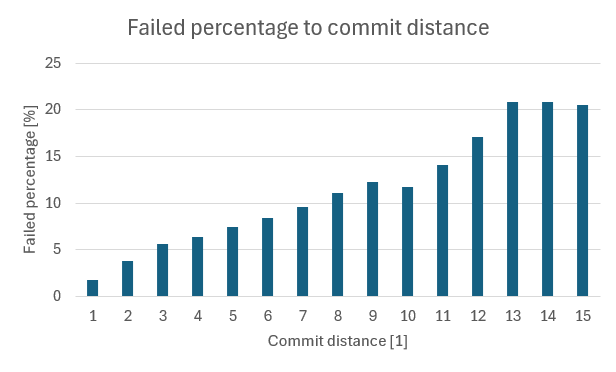
\includegraphics[width=\textwidth]{../img/failure_percentage_graph.png}
    \caption{Graf počtu testů, které selhaly, vůči vzdálenosti commitů v~čase}
\end{figure}

K~tomuto postupnému růstu poměru selhávajících testů dochází, protože se zhoršení výkonu může kumulovat skrze více commitů.
Pokud se tedy měřená metoda zhoršuje v průběhu času, tak se to projeví až u commitu, který tuto metodu dostatečně zesiluje.
Po dostatečném zesílení tohoto zhoršení se metoda zhorší natolik, že ji porovnání se~vzdálenou předchozí verzí detekuje, ačkoli
porovnání s~přímým sousedem by ji nedetekoval.

Ukazuje se tedy, že pomocí PerfEvalu je sice možné detekovat zhoršení výkonu v~rámci průběžné integrace.
Není ale vhodné jej používat jako blokující faktor při integraci. PerfEval by měl být spíše používán jako nástroj
pro detekci zhoršení výkonu v~průběhu vývoje. V~případě, že PerfEval detekuje zhoršení výkonu, tak je uživatel
schopen jednoduše zjistit, kde ke zhoršení došlo. Pokud by PerfEval byl součástí průběžné integrace jako blokující faktor,
tak by se mohlo stát, že by integrace byla zablokovaná kvůli zhoršení výkonu, který ve~skutečnosti z~větší části způsobil jiný commit.

V~grafu na obrázku 6.1 je vidět, že se zde nachází i~několik neúspěšných testů u~commitů se vzdáleností 1.
Tato porovnání byla provedena tak, že se z vybraných 16 commitů vždy vybral commit a jeho soused v tomto
výběru a ne pouze bezprostřední soused. Proto i když bylo výše uvedeno, že PerfEval nezaznamenal žádné zhoršení,
tak na grafu je vidět, že některé testy selhaly. Tato selhání byla způsobena tím, že se výkonnostní testy
se ve skutečnosti porovnávaly i~s~commity, které byly vzdáleny o~víc než jeden commit. To je způsobeno tím,
že výběr commitů byl proveden tak, že byly vybrány commity, které obsahovaly slovo „performance“ v~commit message
a~jejich sousední commity. Celý tento výběr však nejsou bezprostředně navazující commity.

Tato ukázka práce systému PerfEval netvrdí, že se výkon v~projektu Crate zhoršuje.
U~některých metod bylo zaznamenáno také zlepšení. Zlepšování výkonu softwaru totiž bývá
často něco za něco. Zlepšení výkonu jedné metody může znamenat zhoršení výkonu jiné metody.
Získané zlepšení ale může být v~některých případech tak velké, že zhoršení výkonu jiné metody
je přijatelné. PerfEval tedy může být použit jako nástroj pro detekci těchto změn výkonu,
není ale schopen v~schopen se rozhodnout zdali je změna výkonu pozitivní, nebo negativní.

\chapter{Závěr}
%\addcontentsline{toc}{chapter}{Závěr}

Tato práce se snaží navázat na využívání unit testů při vývoji softwaru.
Nástroj PerfEval, který byl vytvořen, má za úkol poskytnout vývojářům možnost
psát výkonnostní testy obdobně jako unit testy.

V první kapitole bylo vysvětleno, co je průběžná integrace. Dále byl popsán scénář programátora, který
ji využívá pro udržování korektnosti svého kódu, a~jak by ji chtěl využít i~pro udržování výkonu.
Programátor měl napsané výkonnostní testy pomocí benchmarkovacího frameworku a~potřeboval je vyhodnocovat.
Neměl ale žádný nástroj, který by uměl výsledky měření porovnat a~vyhodnotit změnu výkonu.

Druhá kapitola se věnuje analýze problematiky kolem vyhodnocování výkonu softwaru. Je zde popsáno jak vypadají výstupy benchmarkovacích frameworků
JMH a BenchmarkDotNET. Dále jsou popsány statistické metody, které se následně v~nástroji využívají k~porovnání
výsledků měření.

Ve třetí kapitole je vysvětleno několik důležitých rozhodnutí, které byly provedeny před a~v~průběhu vývoje nástroje PerfEval.
Zároveň byla nastíněna architektura nástroje a~jakým způsobem se používá.

Uživatelská dokumentace ukazuje jaké příkazy má uživatel k~dispozici včetně jejich argumentů.
V~této kapitole se také uživatel dozví jak nástroj instalovat a~používat včetně toho, jak jej konfigurovat.

Programátorská dokumentace obsahuje detailní popis struktury kódu. Je zde popsáno jaké byly využité návrhové vzory
a~jak spolu jednotlivé třídy vzájemně interagují.

Výsledkem práce je nástroj PerfEval jehož způsob použití včetně nasazení v~rámci existujícího projektu je demonstrováno
v~poslední kapitole. Nástroj byl nasazen v~rámci projektu Crate a~byl použit k~analýze výkonnostních testů verzí, které byly
označené, jako verze se změnou výkonu.

Ukázalo se, že vyvinutý nástroj PerfEval je schopen detekovat změny výkonu. Při použití v~rámci
průběžné integrace je vhodné dodávat verzi, která bude považovaná za~referenční. Tato verze by měla
mít výkon, který chce uživatel udržet. V~případě, že se výkon změní, tak PerfEval uživatele upozorní.
Zároveň tento nástroj splňuje požadavek, že se má připodobnit k~používání unit testů.

Tento nástroj tedy řeší původní programátorův problém chybějícího nástroje pro vyhodnocování výkonu.
Dodáním řádku do svého měřícího skriptu programátor předá informace o~výsledcích měření nástroji PerfEval.
Následně programátor jedním příkazem vyhodnotí změnu mezi požadovanými verzemi.

Do~budoucna by bylo možné nástroj rozšířit například o~vyhodnocování výkonu na bázi skóre.
Optimalizace výkonu totiž obvykle bývá taková, že zlepšením výkonu jednoho testu se zhorší výkon jiného.
Proto by se jednotlivým testům mohlo přiřazovat skóre, které by bylo závislé na změně výkonu a~na tom, jak moc je test důležitý.

%%% Seznam použité literatury
%%% Seznam použité literatury (bibliografie)
%%%
%%% Pro vytváření bibliografie používáme bibTeX. Ten zpracovává
%%% citace v textu (např. makro \cite{...}) a vyhledává k nim literaturu
%%% v souboru literatura.bib.
%%%
%%% Příkaz \bibliographystyle určuje, jakým stylem budou citovány odkazy
%%% v textu. V závorce je název zvoleného souboru .bst. Styly plainnat
%%% a unsrt jsou standardní součástí latexových distribucí. Styl czplainnat
%%% je dodáván s touto šablonou a bibTeX ho hledá v aktuálním adresáři.

\bibliographystyle{czplainnat}    %% Autor (rok) s českými spojkami
% \bibliographystyle{plainnat}    %% Autor (rok) s anglickými spojkami
% \bibliographystyle{unsrt}       %% [číslo]

\renewcommand{\bibname}{Seznam použité literatury}

%%% Vytvoření seznamu literatury. Pozor, pokud jste necitovali ani jednu
%%% položku, seznam se automaticky vynechá.

\bibliography{literatura}

%%% Kdybyste chtěli bibliografii vytvářet ručně (bez bibTeXu), lze to udělat
%%% následovně. V takovém případě se řiďte normou ISO 690 a zvyklostmi v oboru.

% \begin{thebibliography}{99}
%
% \bibitem{lamport94}
%   {\sc Lamport,} Leslie.
%   \emph{\LaTeX: A Document Preparation System}.
%   2. vydání.
%   Massachusetts: Addison Wesley, 1994.
%   ISBN 0-201-52983-1.
%
% \end{thebibliography}


%%% Obrázky v bakalářské práci
%%% (pokud jich je malé množství, obvykle není třeba seznam uvádět)
\listoffigures

%%% Tabulky v bakalářské práci (opět nemusí být nutné uvádět)
%%% U matematických prací může být lepší přemístit seznam tabulek na začátek práce.
\listoftables

%%% Použité zkratky v bakalářské práci (opět nemusí být nutné uvádět)
%%% U matematických prací může být lepší přemístit seznam zkratek na začátek práce.
\chapwithtoc{Seznam použitých zkratek}

%%% Přílohy k bakalářské práci, existují-li. Každá příloha musí být alespoň jednou
%%% odkazována z vlastního textu práce. Přílohy se číslují.
%%%
%%% Do tištěné verze se spíše hodí přílohy, které lze číst a prohlížet (dodatečné
%%% tabulky a grafy, různé textové doplňky, ukázky výstupů z počítačových programů,
%%% apod.). Do elektronické verze se hodí přílohy, které budou spíše používány
%%% v elektronické podobě než čteny (zdrojové kódy programů, datové soubory,
%%% interaktivní grafy apod.). Elektronické přílohy se nahrávají do SISu a lze
%%% je také do práce vložit na CD/DVD. Povolené formáty souborů specifikuje
%%% opatření rektora č. 72/2017.
\appendix
\chapter{Přílohy}

\section{První příloha}

\openright
\end{document}
